\documentclass[11pt]{article}
\usepackage[T1]{fontenc}
\usepackage{lmodern}
\usepackage[margin=1in]{geometry}
\usepackage{amsmath,amssymb,amsthm,mathtools}
\usepackage{bm}
\usepackage{graphicx}
\graphicspath{{figures/}{paper/figures/}}
\usepackage{tikz}
\usetikzlibrary{arrows.meta}
\usepackage{xcolor}
\usepackage{enumitem}
\usepackage{csquotes}
\usepackage[american]{babel}
\usepackage{array,booktabs}
\usepackage{float}
\usepackage{microtype}
\usepackage{hyperref}
\hypersetup{hidelinks,
  pdftitle={Asymptotic-polygon global inversion for planar saturating ridge
    networks and an injective neural-Jacobian separation witness},
  pdfauthor={Logan M. Dixon}}
\usepackage{xurl}
\emergencystretch=3em
\hyphenation{co-di-men-sion homeo-morphism}

\usepackage{aliascnt}
\theoremstyle{plain}
\newtheorem{theorem}{Theorem}[section]
\newaliascnt{proposition}{theorem}
\newtheorem{proposition}[proposition]{Proposition}
\aliascntresetthe{proposition}
\newaliascnt{lemma}{theorem}
\newtheorem{lemma}[lemma]{Lemma}
\aliascntresetthe{lemma}
\newaliascnt{corollary}{theorem}
\newtheorem{corollary}[corollary]{Corollary}
\aliascntresetthe{corollary}
\newaliascnt{conjecture}{theorem}
\newtheorem{conjecture}[conjecture]{Conjecture}
\aliascntresetthe{conjecture}
\newaliascnt{hypothesis}{theorem}
\newtheorem{hypothesis}[hypothesis]{Hypothesis}
\aliascntresetthe{hypothesis}
\theoremstyle{definition}
\newaliascnt{definition}{theorem}
\newtheorem{definition}[definition]{Definition}
\aliascntresetthe{definition}
\newaliascnt{question}{theorem}
\newtheorem{question}[question]{Question}
\aliascntresetthe{question}
\theoremstyle{remark}
\newaliascnt{remark}{theorem}
\newtheorem{remark}[remark]{Remark}
\aliascntresetthe{remark}
\usepackage[capitalize,noabbrev]{cleveref}
\crefname{proposition}{proposition}{propositions}
\Crefname{proposition}{Proposition}{Propositions}
\crefname{lemma}{lemma}{lemmas}
\Crefname{lemma}{Lemma}{Lemmas}
\crefname{corollary}{corollary}{corollaries}
\Crefname{corollary}{Corollary}{Corollaries}
\crefname{conjecture}{conjecture}{conjectures}
\Crefname{conjecture}{Conjecture}{Conjectures}
\crefname{hypothesis}{hypothesis}{hypotheses}
\Crefname{hypothesis}{Hypothesis}{Hypotheses}
\crefname{definition}{definition}{definitions}
\Crefname{definition}{Definition}{Definitions}
\crefname{question}{question}{questions}
\Crefname{question}{Question}{Questions}
\crefname{remark}{remark}{remarks}
\Crefname{remark}{Remark}{Remarks}

\newcommand{\R}{\mathbb{R}}
\newcommand{\sgn}{\operatorname{sgn}}
\newcommand{\norm}[1]{\lVert #1 \rVert}
\newcommand{\clinf}{C_{\infty}}
\newcommand{\Wder}{\mathcal{W}_{B,c}}
\newcommand{\wind}{\operatorname{wind}}
\DeclareMathOperator{\Ker}{ker}

\title{Asymptotic-polygon global inversion for planar saturating ridge networks
and an injective neural--Jacobian separation witness%
\thanks{Prompted by the Neural Jacobian Conjecture of Chen and Jiang,
\href{https://arxiv.org/abs/2606.10806}{arXiv:2606.10806}.}}
\author{Logan M. Dixon\thanks{Independent Researcher. Email:
\texttt{lmdixon23@gmail.com}. ORCID: 0009-0001-0592-462X.}}
\date{September 2026}

\begin{document}
\maketitle

\begin{abstract}
For sigmoid ridge networks $F(x)=A\sigma(Bx+c)$, local Jacobian orientation and global multiplicity are governed by different finite-dimensional geometries.  We study an explicit $n=2$, $N=4$ network with $\det DF>0$ on $\R^2$ whose segment-averaged Jacobian has negative determinant at one pair and is singular at an intermediate pair, so the classical mean-value univalence certificate fails.  The same network is nevertheless a global diffeomorphism onto an explicit nonconvex octagon.  Two finite-dimensional geometries explain the separation.  In the interior, $\det DF$ is an indefinite quadratic form evaluated on the nonlinear derivative-weight image $\{\sigma'(Bx+c):x\in\R^2\}$; a convexity and optimally weighted AM--GM argument proves positivity there by one rigorously enclosed scalar inequality.  At infinity, the row arrangement of $B$ produces a signed-column polygon whose winding number determines the exact number of preimages.  A uniform large-circle approximation yields the formula $\#F^{-1}(y)=\operatorname{sgn}(\det DF)\,\wind(\gamma,y)$ off the boundary loop, and hence a necessary and sufficient planar injectivity criterion.  Exact sign-plus-magnitude polygon criteria and validated parameter certificates show that the witness mechanism persists on an explicit open neighborhood.  Thus averaged-Jacobian univalence is strictly stronger than actual injectivity, and the asymptotic winding supplies the decisive global certificate for this separation witness.
\end{abstract}

\medskip
\noindent\textbf{2020 Mathematics Subject Classification.} 26B10 (primary); 57N05, 65G20, 68T07, 15A15.

\smallskip
\noindent\textbf{Keywords.} global injectivity; sigmoid ridge network; Neural Jacobian Conjecture; cluster set at infinity; Jordan curve; Schoenflies theorem; asymptotic polygon; validated numerics.

% =====================================================================
\section{Introduction}\label{sec:intro}
Does an everywhere-nonsingular Jacobian force a smooth map to be globally injective? Chen and Jiang formulated this question for sigmoid ridge networks $F(x)=A\sigma(Bx+c)$ as the Neural Jacobian Conjecture~\cite{chen-jiang}.  It holds at hidden widths $N\in\{n,n+1\}$; Chen and Jiang report proofs for $N=n+1$~\cite{chen-jiang}, and \Cref{thm:closedwidths} gives a short graph-coordinate proof that also exposes a coordinate dependence hidden by the usual mean-value route. The present paper studies the first higher width, $n=2$, $N=4$, but does not claim to settle the unrestricted conjecture at that width.

Classical global-inversion theory obtains one-to-one behavior from properness, covering-space continuation, or quantitative derivative conditions \cite{gutu-jaramillo,ruzhansky-sugimoto}; neural-network injectivity has also been studied for other activation and architecture classes, including sharp results for ReLU networks~\cite{puthawala}.  The bounded saturating ridge setting considered here has a different geometry because escape to infinity produces a finite boundary object rather than an unbounded or piecewise-linear range.

The paper opens with an explicit $n=2$, $N=4$ network for which the mean-value route fails.  This network has $\det DF>0$ certified on all of $\R^2$ but a \emph{negative} segment-averaged Jacobian determinant at an explicit pair --- a certified \emph{separation example}, on which the mean-value univalence certificate provably fails. Injectivity of that network cannot be inferred from this calculation: a sign-vector analysis~\cite{mhr} narrows any collision to two open sectors but does not exclude it.  We prove that the map is injective by analyzing its boundary at infinity.

The witness, its pointwise positivity certificate, and its negative and singular segment averages are stated here in full, so the separation result is self-contained. The contribution of the paper is to settle the injectivity of that witness and to develop the general boundary geometry that does so.

\begin{quote}\emph{The canonical witness $F(x)=A\sigma(Bx+c)$ is a global $C^1$ diffeomorphism of $\R^2$ onto an explicit open octagon; in particular it is injective} (\Cref{cor:injective}).\end{quote}

\paragraph{Two finite geometries.} The argument separates local orientation from global multiplicity.  With $z=Bx+c$, $w=\sigma'(z)$, and $m_{ij}=\det(A_{\{i,j\}})\det(B_{\{i,j\}})$, define $Q_M(w)=\sum_{i<j}m_{ij}w_iw_j$.  The proof architecture is
\[
\begin{array}{ccccc}
x &\longmapsto& z=Bx+c &\longmapsto&
w=\sigma'(z)\longmapsto Q_M(w)=\det DF(x),\\[3pt]
u\in S^1 &\longmapsto& \text{tope of the row arrangement}
&\longmapsto& \gamma(u)=A\,s(u)\longmapsto \wind(\gamma,\cdot).
\end{array}
\]
The upper line controls pointwise orientation on a constrained derivative-weight surface; the lower line controls the global sheet number through an asymptotic boundary loop.  Segment averaging may leave the derivative-weight image and cross the zero cone of $Q_M$ without changing the winding data that enforce injectivity.  This interior--boundary factorization is the organizing principle of the paper.

The injectivity proof does not rely on the averaged Jacobian.  It begins with a general planar principle (\Cref{thm:main}): a bounded local homeomorphism whose limit values at infinity lie on a Jordan curve is a homeomorphism onto the region that curve bounds.  For a saturating ridge network those limit values lie on an explicit \emph{asymptotic polygon} whose directed edges are signed columns of $A$, ordered by the row arrangement of $B$ (\Cref{lem:polygon,prop:normal-form}). The remaining question is therefore finite but not merely computational: when is that prescribed centrally symmetric polygon simple?

The paper answers that question at three levels.  A complete orientation formula reduces simplicity, including degenerate cases, to finitely many polynomial sign and interval-order predicates (\Cref{thm:closed-form}).  In the sign-coherent regime, the mixed minors $\det(a_i,a_j)\det(b_i,b_j)$ have one sign exactly when the asymptotic polygon is strictly convex (\Cref{thm:mixed-convexity}).  Beyond that regime, magnitudes are indispensable: positive rescaling can preserve every determinant sign while changing a simple polygon into a self-intersecting one (\Cref{prop:sign-insufficient}).  A short magnitude-sensitive criterion then proves the witness octagon simple from four monotonicity signs and three prefix-side signs (\Cref{thm:one-sided,cor:witness-structural}); the twenty-pair exact segment test is retained only as a cross-check.

These strict inequalities also show that polygon simplicity is stable under small perturbations. Combined with the analytic determinant theorem and the separately implemented finite parameter certificates, this yields both a human-readable analytic class and a certified neighborhood of globally injective networks around the witness (\Cref{cor:analytic-class,thm:open-family}). The explicit certified boxes remain local in parameter space, while the analytic criterion itself defines a broader open subclass. The analytic and geometric hypotheses are sufficient conditions for this open subclass; no necessity claim for all four-ridge networks is made here.

\Cref{sec:weights} develops the derivative-weight formulation and analytic positivity mechanism; \Cref{sec:theorem} proves the cluster-set inversion theorem; \Cref{sec:lemma} derives the asymptotic polygon; \Cref{sec:simplicity} develops the structural criteria needed for the witness; \Cref{sec:cert} applies them; and \Cref{sec:injectivity,sec:winding} establish global injectivity and the exact multiplicity formula. \Cref{sec:n4} records the remaining four-ridge boundary obstruction, while \Cref{sec:reconcile,sec:conclusion} synthesize the interior and boundary mechanisms. Complete all-cases polygon predicates and quantitative certificate details are collected in \Cref{app:polygon-criteria,app:det}.

% =====================================================================
\section{The certified separation witness}\label{sec:separation}

Let $\sigma(t)=(1+e^{-t})^{-1}$.  The canonical matrices $A\in\R^{2\times4}$, $B\in\R^{4\times2}$ and bias $c\in\R^4$ are stored in \path{data/witness.json}; their displayed decimal tokens are treated as exact rationals by every certificate.  For
\[
 DF(x)=A\operatorname{diag}\!\bigl(\sigma'(Bx+c)\bigr)B,
\]
Cauchy--Binet gives
\[
 \det DF(x)=\sum_{0\le i<j<4}m_{ij}\,
 \sigma'(b_i\cdot x+c_i)\sigma'(b_j\cdot x+c_j),
 \qquad
 m_{ij}=\det(A_{ij})\det(B_{ij}).
\]
Five $m_{ij}$ are positive and $m_{23}<0$.

\begin{theorem}[certified separation at the first open width]
\label{thm:separation}
For the canonical $n=2,N=4$ witness:
\begin{enumerate}[label=(\roman*),leftmargin=*]
\item $\det DF(x)>0$ for every $x\in\R^2$;
\item for $p=(-2.76601947,12)$ and $q=(7.08288117,12)$,
\[
 \det\overline{DF}(p,q)<-1.7199\times10^{-5},
 \qquad
 \overline{DF}(p,q)=\int_0^1DF(p+t(q-p))\,dt;
\]
\item there exists $t_*\in(0,1)$ such that $\det\overline{DF}(p,p+t_*(q-p))=0$.
\end{enumerate}
Thus pointwise Jacobian positivity does not imply the averaged-Jacobian nonsingularity hypothesis used by the standard mean-value univalence route.  By \Cref{cor:injective} the witness is nevertheless injective, so the criterion of \Cref{lem:mv} is strictly stronger than injectivity.  It is strictly stronger already at the closed width $N=n+1$ (\Cref{prop:coorddep}); what is specific to width $n+2$ is that the determinant ceases to be affine in a single varying slot, so the graph-coordinate rank-one commutation used at width $n+1$ no longer applies.
\end{theorem}

\begin{proof}
Part (i) is proved analytically for the witness by \Cref{prop:analytic-det}; the validated compact-plus-tail certificate (\Cref{app:det}) corroborates it through a separate interval implementation and certifies the parameter boxes. For (ii), each diagonal divided difference is evaluated from the closed sigmoid formula and the resulting $2\times2$ determinant is enclosed with directed rounding. The global analytic proof, separately corroborated by the compact-plus-tail certificate, also establishes pointwise determinant positivity along the displayed segment. At the coincident endpoint, $\overline{DF}(p,p)=DF(p)$ has positive determinant; continuity of the averaged matrix in the endpoint and (ii) give (iii) by the intermediate value theorem.
\end{proof}

\begin{remark}
\Cref{thm:separation} alone does not decide injectivity: a collision forces a singular segment average, but the converse fails. The remainder of the paper proves injectivity of this witness and develops the boundary geometry that supplies the missing global certificate.
\end{remark}


% =====================================================================
\section{The mean-value certificate and the closed widths}\label{sec:closedwidth}

This section fixes the certificate whose failure the paper studies, records the
classical argument that closes the two lowest widths, and isolates a
coordinate dependence that the classical argument conceals.

\begin{lemma}[mean-value univalence; folklore]\label{lem:mv}
Let $\Omega\subseteq\R^n$ be open and convex and $G\in C^1(\Omega,\R^n)$.  If
the averaged Jacobian
$\overline{DG}(x,y)=\int_0^1 DG\bigl(y+t(x-y)\bigr)\,dt$
is nonsingular for all $x,y\in\Omega$, then $G$ is injective.
\end{lemma}

\begin{proof}
Applying the fundamental theorem of calculus componentwise along the segment
from $y$ to $x$, which lies in $\Omega$ by convexity, gives
$G(x)-G(y)=\overline{DG}(x,y)(x-y)$.  Nonsingularity forces $x=y$ whenever
$G(x)=G(y)$.
\end{proof}

\begin{theorem}[widths $N=n$ and $N=n+1$]\label{thm:closedwidths}
Every $F(x)=A\sigma(Bx+c)$ with $N\le n+1$ and $\det DF$ nowhere zero on
$\R^n$ is injective.
\end{theorem}

\begin{proof}
Since $DF=A\operatorname{diag}(\sigma'(Bx+c))B$ is nonsingular and the middle
factor is a positive diagonal, $\operatorname{rank}A=\operatorname{rank}B=n$;
in particular $N\ge n$ and some $n$ rows of $B$ are independent.  Permute the
hidden units so that the first $n$ rows form an invertible $B_1$ and set
$y=B_1x+c_1$, an invertible affine change of the source.  The first $n$
preactivations are then $y_1,\dots,y_n$.

If $N=n$ the map becomes $y\mapsto A\sigma(y)$ with $A$ invertible, and
$\sigma$ is a strictly increasing bijection $\R\to(0,1)$ applied
coordinatewise, so the composite is injective.

If $N=n+1$ the remaining preactivation is an affine function
$\ell(y)=a^{\mathsf T}y+\beta$, and
$F=C\sigma(y)+w\,\sigma(\ell(y))$ with $C\in\R^{n\times n}$, $w\in\R^n$.
Substitute $u=\sigma(y)$.  Because $\sigma$ is a diffeomorphism of $\R$ onto
$(0,1)$, this is a diffeomorphism of $\R^n$ onto the open cube $(0,1)^n$, and
injectivity of $F$ is equivalent to injectivity of
\[
 T(u)=Cu+w\,h(u),\qquad h(u)=\sigma\bigl(\ell(\sigma^{-1}(u))\bigr),
\]
on $(0,1)^n$, which is open and convex.  Here
$DT(u)=C+w\,\nabla h(u)^{\mathsf T}$, so $\det DT$ is an affine function of
$\nabla h$.  Affine functions commute with averaging, whence
\[
 \det\overline{DT}(u,v)=\int_0^1\det DT\bigl(v+t(u-v)\bigr)\,dt .
\]
The integrand is continuous and nowhere zero on the connected set $(0,1)^n$,
hence of constant sign, so the integral is nonzero and
\Cref{lem:mv} applies to $T$.
\end{proof}

\begin{remark}[the mechanism, and where it lives]\label{rmk:mechanism}
The proof succeeds because at kernel dimension one the determinant is affine
in the single varying slot, so determinant and averaging commute.  At kernel
dimension two the determinant is genuinely multilinear and the commutation can
fail; that is the obstruction this paper exhibits at $N=n+2$.

The commutation above holds along straight segments in the \emph{graph}
coordinate $u=\sigma(y)$.  Straight segments in $x$ are not carried to
straight segments in $u$, so \Cref{thm:closedwidths} does not assert that the
averaged Jacobian in the original coordinate is nonsingular.
\Cref{prop:coorddep} shows that it need not be, already at $N=n+1$.
\end{remark}

\begin{remark}[scope]\label{rmk:scope}
For $n=1$ and every width, $\det DF>0$ means $F'>0$, so $F$ is strictly
increasing and injective.  The regime left open by \Cref{thm:closedwidths} is
therefore $n\ge2$ and $N\ge n+2$.
\end{remark}

\subsection{Coordinate dependence of the averaged-Jacobian criterion}

The certificate of \Cref{lem:mv} is stronger than injectivity, and strictly so
already where injectivity is guaranteed.

\begin{proposition}[coordinate dependence at the closed width]\label{prop:coorddep}
Let $n=2$, $N=3$ and
\[
 A=\begin{pmatrix} 0 & 1 & -10\\ 1 & 0 & -10\end{pmatrix},\qquad
 B=\begin{pmatrix} 1 & 0\\ 0 & 1\\ 3/10 & 3/10\end{pmatrix},\qquad c=0 .
\]
Then $F(x)=A\sigma(Bx+c)$ satisfies $\det DF>0$ on $\R^2$ and is a global
diffeomorphism onto an open hexagon, yet there are $p,q$ with
$\det\overline{DF}(p,q)<0$, hence an intermediate pair at which
$\overline{DF}$ is singular.  The hypothesis of \Cref{lem:mv} therefore fails
in the original coordinate at width $N=n+1$.  It cannot fail at width $N=n$,
where $\det\overline{DF}=\det A\,\det B\prod_i\delta_i$ carries the fixed sign
of $\det A\det B$.
\end{proposition}

\begin{proof}
The mixed minors are $m_{01}=-1$, $m_{02}=m_{12}=3$, so by Cauchy--Binet
$\det DF=-\rho_0\rho_1+3\rho_0\rho_2+3\rho_1\rho_2$ with
$\rho_i=\sigma'(z_i)$ and $z_2=\tfrac3{10}(z_0+z_1)$.  Dividing by
$\rho_0\rho_1>0$, positivity is equivalent to $R>1$ where
$R=3\rho_2(\rho_0^{-1}+\rho_1^{-1})$.  Using
$\sigma'(t)^{-1}=2+2\cosh t$,
\[
 R=3\,\frac{2+\cosh z_0+\cosh z_1}{1+\cosh\bigl(\tfrac3{10}(z_0+z_1)\bigr)} ,
\]
so $R\ge6$ is equivalent to
$\cosh z_0+\cosh z_1\ge 2\cosh\bigl(\tfrac3{10}(z_0+z_1)\bigr)$.  Now
\[
 \cosh z_0+\cosh z_1
 =2\cosh\tfrac{z_0+z_1}{2}\,\cosh\tfrac{z_0-z_1}{2}
 \ \ge\ 2\cosh\tfrac{z_0+z_1}{2}
 \ \ge\ 2\cosh\bigl(\tfrac3{10}(z_0+z_1)\bigr),
\]
the first step because $\cosh\ge1$ and the second because
$\tfrac3{10}<\tfrac12$ and $\cosh$ is even and increasing on $[0,\infty)$.
Equality forces $z_0=z_1$ and $z_0+z_1=0$, so $R\ge6$ with equality only at
the origin, and $\det DF\ge5\rho_0\rho_1>0$ everywhere.

For the failure take $p=(-40,120)$ and $q=(40,-20)$.  The three divided
differences are
$\delta_i=\bigl(\sigma(t_i(q))-\sigma(t_i(p))\bigr)/\bigl(t_i(q)-t_i(p)\bigr)$
with preactivation segments $[-40,40]$, $[120,-20]$ and $[24,6]$.  Since
$1-\sigma(t)=\sigma(-t)<e^{-t}<2^{-t}$ for $t>0$, and in particular
$2^{-39}<10^{-3}$ and $2^{-20}+2^{-120}<10^{-3}$, one has
\[
 \delta_0>\frac{999}{80000},\qquad
  \delta_1>\frac{999}{140000},\qquad
  \delta_2<\frac1{1152},
 \]
while trivially $\delta_0<1/80$ and $\delta_1<1/140$.  Therefore
\[
\det\overline{DF}(p,q)
 =-\delta_0\delta_1+3\delta_2(\delta_0+\delta_1)
 <-\frac{998001}{11200000000}+\frac{11}{215040}
 =-\frac{182179}{4800000000}<0.
 \]
(Direct evaluation gives approximately $-8.1191\times10^{-5}$.)  At the
coincident pair $\overline{DF}(p,p)=DF(p)$ has positive determinant, and
$\overline{DF}(p,p+s(q-p))$ is continuous in $s$, so some intermediate pair is
singular.

Finally the rows of $B$ are pairwise nonparallel, so \Cref{lem:polygon}
applies.  In cyclic order the asymptotic polygon has the six distinct integer
vertices $(-9,-9)$, $(-9,-10)$, $(1,0)$, $(0,0)$, $(0,1)$, $(-10,-9)$.
They form a centrally symmetric hexagon with signed area $19$; exact integer
orientation predicates show it is simple, and its winding spectrum is
$\{0,1\}$.  \Cref{thm:main} gives that $F$ is a global diffeomorphism onto the
bounded component, and \Cref{cor:iff} gives injectivity independently of
\Cref{thm:closedwidths}.
\end{proof}

\begin{remark}
The boundary for original-coordinate mean-value failure is therefore between
$N=n$ and $N=n+1$.  It is a different boundary from the one separating the
settled and unsettled widths of the injectivity question itself, and the two
should not be conflated.
\end{remark}

% =====================================================================
\section{Derivative-weight geometry and analytic positivity}\label{sec:weights}

Put $\rho=\sigma'$ and, for $z=Bx+c$, define the derivative-weight vector
\[
 w(x)=\rho(z)=\bigl(\rho(z_0),\ldots,\rho(z_{N-1})\bigr),
 \qquad
 \Wder=\{w(x):x\in\R^2\}.
\]
For the mixed coefficients $m_{ij}=\det(A_{\{i,j\}})\det(B_{\{i,j\}})$, let
\[
 Q_M(w)=\sum_{i<j}m_{ij}w_iw_j.
\]
Cauchy--Binet gives the exact factorization
\begin{equation}\label{eq:weight-factorization}
 \det DF(x)=Q_M(w(x)).
\end{equation}
Thus pointwise Jacobian positivity asks for positivity of a generally indefinite quadratic form only on the nonlinear image $\Wder$, not on the whole positive orthant.

\begin{proposition}[pointwise and averaged derivative weights]\label{prop:weight-average}
For a segment $x_t=p+t(q-p)$, set $\bar w=\int_0^1w(x_t)\,dt$.  Then
\[
 \overline{DF}(p,q):=\int_0^1DF(x_t)\,dt
 =A\operatorname{diag}(\bar w)B,
 \qquad
 \det\overline{DF}(p,q)=Q_M(\bar w).
\]
Consequently, pointwise positivity controls $Q_M$ on $\Wder$, whereas the mean-value certificate tests path barycenters in $\operatorname{conv}(\Wder)$.
\end{proposition}
\begin{proof}
The matrices $A$ and $B$ are constant along the segment, so integration commutes with the diagonal derivative factor.  The determinant identity is again Cauchy--Binet.
\end{proof}

For logistic activation, $\rho(t)=\tfrac14e^{-\psi(t)}$ with $\psi(t)=2\log\cosh(t/2)$.  The function $\psi$ is even, convex, and nonnegative.  The next result gives a human-readable positivity class in the one-negative-minor regime.

Assume $m_{23}<0$, $m_{02},m_{03}>0$, and all remaining mixed coefficients are nonnegative.  Write
\[
 b_0=\alpha b_2+\beta b_3,\qquad
 \delta=c_0-\alpha c_2-\beta c_3,
\]
put $a=|\alpha|$, $b=|\beta|$, $r=1-a-b$, and assume $r>0$.  For $\mu\in I:=[a,1-b]$, set $\lambda=1-\mu$ and
\[
 G(\mu)=
 \left(\frac{m_{02}}{1-\mu}\right)^{1-\mu}
 \left(\frac{m_{03}}{\mu}\right)^{\mu}.
\]
The strictly concave function $\log G$ has unconstrained maximizer $\mu_0=m_{03}/(m_{02}+m_{03})$.  Hence the optimal admissible weight is
\begin{equation}\label{eq:optimal-mu}
 \mu_* = \min\!\left\{1-b,\max\!\left\{a,
 \frac{m_{03}}{m_{02}+m_{03}}\right\}\right\},
 \qquad \lambda_*=1-\mu_*.
\end{equation}
If $\mu_0\in I$, then $G(\mu_*)=m_{02}+m_{03}$.

\begin{proposition}[analytic one-negative-minor dominance]\label{prop:analytic-det}
Under the preceding hypotheses, if
\begin{equation}\label{eq:analytic-dominance}
 G(\mu_*)\exp\!\left[-r\psi\!\left(\frac{\delta}{r}\right)\right]
 >|m_{23}|,
\end{equation}
then $\det DF(x)>0$ for every $x\in\R^2$.
\end{proposition}
\begin{proof}
For any admissible $\mu\in I$ and $\lambda=1-\mu$, the affine relation gives $z_0=\alpha z_2+\beta z_3+\delta$.  Convexity and evenness imply
\[
 \psi(z_0)\le a\psi(z_2)+b\psi(z_3)+r\psi(\delta/r),
\]
and therefore
\[
 -\psi(z_0)+\mu\psi(z_2)+\lambda\psi(z_3)
 \ge-r\psi(\delta/r).
\]
Weighted AM--GM applied to $X=m_{02}\rho(z_0)/\rho(z_3)$ and $Y=m_{03}\rho(z_0)/\rho(z_2)$ yields
\[
 X+Y\ge G(\mu)\exp[-r\psi(\delta/r)].
\]
After dividing the Cauchy--Binet expansion by $\rho(z_2)\rho(z_3)>0$ and discarding the remaining nonnegative terms, maximizing over $I$ gives \eqref{eq:analytic-dominance} and strict positivity.
\end{proof}

\begin{remark}[relation to relative-entropy certificates]\label{rmk:sage}
The proof is a one-negative-term arithmetic--geometric-mean certificate.  In signomial optimization this mechanism is formalized by AGE/SAGE and relative entropy methods~\cite{chandrasekaran-shah}; here the row circuit restricts the logits strongly enough that the certificate reduces to the scalar optimization \eqref{eq:optimal-mu}.
\end{remark}

\begin{corollary}[analytic global-injectivity class]\label{cor:analytic-class}
Let $F(x)=A\sigma(Bx+c)$ satisfy the hypotheses of \Cref{prop:analytic-det} and the strict inequality \eqref{eq:analytic-dominance}. Assume in addition that the rows of $B$ are nonzero and pairwise nonparallel and that the resulting asymptotic polygon is simple. Then $F$ is a global $C^1$ diffeomorphism onto the bounded Jordan domain enclosed by that polygon.
\end{corollary}
\begin{proof}
\Cref{prop:analytic-det} gives $\det DF>0$ on $\R^2$, so $F$ is a local $C^1$ diffeomorphism, while $\sigma\in(0,1)^N$ makes it bounded. \Cref{lem:polygon} gives $\clinf(F)\subseteq\Gamma$; the assumed simplicity makes $\Gamma$ a Jordan curve, and \Cref{thm:main} applies.
\end{proof}

For the canonical witness, exact rational computation gives $r>0$.  The executable certificate uses the admissible rational weights $\mu=51/1000$, $\lambda=949/1000$ for reproducibility.  Since $G(\mu_*)\ge G(51/1000)$, the rational evaluation gives a rigorous lower bound for the optimized left side of \eqref{eq:analytic-dominance}: it exceeds $0.1290339743302$, while $|m_{23}|<0.1261291706757$.  The margin exceeds $0.0029048036545$. The validated spatial certificate in \Cref{app:det} is therefore separate computational corroboration for the central witness and remains load-bearing only for the explicit parameter boxes.

% =====================================================================
\section{A planar Jordan cluster-set inversion theorem}\label{sec:theorem}

\begin{definition}[cluster set at infinity]\label{def:clinf}
For a map $F:\R^2\to\R^2$, the \emph{cluster set at infinity} is
\[
\clinf(F)=\bigl\{\,y\in\R^2 : \text{there exist } x_k \text{ with }
\norm{x_k}\to\infty \text{ and } F(x_k)\to y \,\bigr\}
=\bigcap_{R>0}\overline{F(\{\,x:\norm{x}>R\,\})}.
\]
\end{definition}

\begin{theorem}[planar Jordan cluster-set inversion]\label{thm:main}
Let $F:\R^2\to\R^2$ be a bounded local homeomorphism, and suppose there is a Jordan curve $\Gamma\subset\R^2$ with $\clinf(F)\subseteq\Gamma$. Let $D$ be the bounded component of $\R^2\setminus\Gamma$. Then $F$ is a homeomorphism of $\R^2$ onto $D$. If moreover $F$ is $C^1$ with $\det DF\neq 0$ everywhere, then $F$ is a $C^1$ diffeomorphism of $\R^2$ onto $D$.
\end{theorem}

The proof (\Cref{app:proof}) runs in five steps.
\begin{enumerate}[label=\textbf{Step \Alph*.},leftmargin=*]
\item \textbf{Relative properness.} For compact $K\subseteq\R^2\setminus\Gamma$, the preimage $F^{-1}(K)$ is closed and bounded, hence compact: an unbounded preimage would force an escaping sequence with a cluster value in $K\cap\Gamma=\varnothing$.
\item \textbf{The image misses the unbounded component $E$.} On $P:=F^{-1}(E)$ the restriction $F|_P$ is open (local homeomorphism) and proper (Step~A), hence closed; so $F(P)$ is open and closed in the connected set $E$. If nonempty it is all of $E$, impossible since $F(\R^2)$ is bounded. Thus $P=\varnothing$.
\item \textbf{The image misses $\Gamma$.} If $F(x_0)\in\Gamma$, openness gives a neighborhood of $F(x_0)$ inside $F(\R^2)$; since $\Gamma=\partial E$, that neighborhood meets $E$, contradicting Step~B. Hence $F(\R^2)\subseteq D$.
\item \textbf{Surjectivity onto $D$.} The map $F:\R^2\to D$ is proper (Step~A), so its image is open and closed in the connected set $D$; being nonempty, it is all of $D$.
\item \textbf{A single sheet.} A proper local homeomorphism onto the locally compact, locally connected space $D$ is a covering map; by Jordan--Schoenflies $D$ is homeomorphic to an open disk, hence simply connected, so a connected covering is trivial and $F$ is a homeomorphism.
\end{enumerate}

\begin{remark}[role of the hypotheses]\label{rmk:sharp}
Boundedness cannot be dropped: the identity map $F(x)=x$ is a local diffeomorphism with $\clinf(F)=\varnothing\subseteq\Gamma$ for any Jordan curve $\Gamma$, yet it is not a homeomorphism onto a bounded component (it maps onto all of $\R^2$). This isolates boundedness, the one failing hypothesis. The containment $\clinf(F)\subseteq\Gamma$ cannot be dropped: a bounded infinite cover of an annulus is a non-injective bounded local diffeomorphism whose cluster set contains interior points. Simplicity of $\Gamma$ cannot be dropped: a self-intersecting limit curve has no well-defined bounded component and defeats Schoenflies.
\end{remark}

% =====================================================================
\section{The asymptotic polygon of a ridge network}\label{sec:lemma}

Write $F(x)=A\,f(Bx+c)$ with columns $a_0,\dots,a_{N-1}\in\R^2$ of $A$ and rows $b_0,\dots,b_{N-1}\in\R^2$ of $B$, and let $f$ act coordinatewise. For a unit vector $u$ put $S(u)=\{\,i: b_i\cdot u>0\,\}$ and $V(S)=\sum_{i\in S}a_i$. The \emph{asymptotic polygon} $\Gamma$ is the closed curve through the vertices $V(S(u))$ ordered by the angular arrangement $\{\,b_i\cdot u=0\,\}$ on the circle; consecutive sectors differ by one flipped index, so each edge is $\pm a_j$.

\begin{lemma}[cluster set of a ridge network]\label{lem:polygon}
Let $f:\R\to\R$ be strictly increasing with $\lim_{t\to-\infty}f(t)=0$ and $\lim_{t\to+\infty}f(t)=1$, and let the nonzero rows $b_i$ be pairwise nonparallel. Then $\clinf(F)\subseteq\Gamma$. Only monotonicity and the two endpoint limits are used; no growth rate is assumed.
\end{lemma}

The proof (\Cref{app:proof}) passes to a limiting direction $x_k/\norm{x_k}\to u$: every index with $b_i\cdot u\neq 0$ saturates to $0$ or $1$ with sign $\sgn(b_i\cdot u)$; pairwise nonparallel rows leave at most one index $j$ with $b_j\cdot u=0$, whose activation subconverges to some $t\in[0,1]$, so the image limit is the edge point $V(S)+t\,a_j$.

\begin{remark}[activation class]\label{rmk:activation}
The inclusion $\clinf(F)\subseteq\Gamma$ holds for every bounded, strictly increasing, saturating activation with limits $0$ and $1$; it is in this sense independent of the activation. It does not extend to unbounded activations such as the rectified linear unit, which violate both the boundedness of $F$ and the finite-limit step.
\end{remark}

\begin{remark}[why simplicity is not automatic]\label{rmk:notzonotope}
The vertices $V(S)$ are subset sums of the \emph{columns} $a_i$, but their cyclic order is fixed by the \emph{row} arrangement $\{\,b_i\cdot u=0\,\}$. Consequently $\Gamma$ is not the boundary of the zonotope generated by the $a_i$ and need not be convex, or even simple; simplicity is a genuine instance-specific condition, verified for the witness in \Cref{sec:cert}.
\end{remark}

% =====================================================================
\section{Classifying simplicity of the asymptotic polygon}\label{sec:simplicity}

Let $i_1,\ldots,i_N$ be the order in which the row separators are crossed along one open semicircle.  Let $\varepsilon_k\in\{\pm1\}$ record whether the $i_k$-th activation switches from its lower to its upper saturation value or in the reverse direction, and put
\[
 g_k=(\ell_+-\ell_-)\varepsilon_k a_{i_k},\qquad
 p_0=0,\qquad p_k=\sum_{r=1}^k g_r,\qquad S=p_N.
\]
For the normalization $\ell_-=0$, $\ell_+=1$ used elsewhere in the paper, the common scalar factor is one.

\begin{proposition}[central-symmetric normal form]\label{prop:normal-form}
After translation, the full asymptotic polygon has directed edge sequence
\[
 g_1,\ldots,g_N,-g_1,\ldots,-g_N
\]
and vertex sequence
\[
 0,p_1,\ldots,p_{N-1},S,S-p_1,\ldots,S-p_{N-1}.
\]
It is therefore centrally symmetric about $S/2$.  If $C=[p_0,p_1,\ldots,p_N]$, the second half of the boundary is the reflected chain $S-C$.
\end{proposition}

\begin{proof}
Antipodal directions reverse every saturation sign, so the second crossing of each separator reverses the first edge.  Summing the first $N$ edges gives $S$; summing the corresponding negatives returns to the origin.  The displayed vertices follow by partial summation, and $x\mapsto S-x$ interchanges the two half-chains.
\end{proof}

\begin{theorem}[chain--reflection classification]\label{thm:chain-reflection}
The asymptotic polygon is a Jordan polygon if and only if $S\neq0$, the chain $C$ is an embedded polygonal arc from $0$ to $S$, and
\[
 C\cap(S-C)=\{0,S\}.
\]
\end{theorem}

\begin{proof}
If $S=0$ the two half-chains share both endpoints and the vertex sequence of \Cref{prop:normal-form} repeats $0$, so the closed curve is not embedded; the condition $S\neq0$ is therefore necessary and is assumed throughout what follows.  Granting it, a simple closed polygon splits at the antipodal vertices $0,S$ into two embedded arcs with disjoint interiors.  Conversely, two embedded arcs with the same two endpoints and otherwise disjoint images have union homeomorphic to a circle.
\end{proof}

A complete all-cases semialgebraic criterion, including collinear and degenerate cases, is recorded in \Cref{app:polygon-criteria}. The main text now turns to the structural regimes that explain the witness.

The formula is complete but does not by itself explain geometry.  The first structural regime is convexity.  Define the mixed minors
\[
 M_{ij}=\det(a_i,a_j)\det(b_i,b_j).
\]

\begin{theorem}[mixed-minor convexity]\label{thm:mixed-convexity}
Assume the rows of $B$ are nonzero and pairwise nonparallel, and the signed edge generators $g_1,\ldots,g_N$ are nonzero and pairwise nonparallel.  The asymptotic polygon is strictly convex if and only if all $M_{ij}$ have the same nonzero sign.
\end{theorem}

\begin{proof}
At the $k$-th crossing let $u_k$ be the unit direction and put $n_k=\varepsilon_k b_{i_k}$.  The derivative of $b_{i_k}\cdot u(\theta)$ has sign $\varepsilon_k$, so $n_k$ is a positive multiple of the positively oriented tangent $u'(\theta_k)$.  Hence $\det(n_k,n_\ell)>0$ for $k<\ell$.  Since
\[
 \det(g_k,g_\ell)\det(n_k,n_\ell)
 = (\ell_+-\ell_-)^2
   \det(a_{i_k},a_{i_\ell})\det(b_{i_k},b_{i_\ell}),
\]
the signs of the pairwise turns among $g_1,\ldots,g_N$ are exactly the signs of the mixed minors.  One common sign means that these generators occur in strict angular order inside an open semicircle; adjoining their negatives gives the strict angular edge order of a centrally symmetric convex polygon.  Conversely, the directed edges of a strictly convex polygon turn strictly in one direction, so all pairwise determinants in its first half, and therefore all mixed minors, have one sign.
\end{proof}

\begin{remark}[topes, chirotopes, circuits, and Pl\"ucker coordinates]
\label{rmk:om-synthesis}
The central row arrangement of $B$ defines a realizable rank-two oriented matroid: its direction sectors are topes, and traversing $S^1$ produces an antipodal cycle in the tope graph that determines the ordered saturation cycle.  The asymptotic polygon is the linear image of that tope cycle under $A$. The signs of the $2\times2$ minors are the rank-two chirotopes, so \Cref{thm:mixed-convexity} says that compatibility of the input and output chirotopes is exactly the convex boundary regime \cite{oriented-matroids}.  The row relation used in \Cref{prop:analytic-det} is a circuit relation and drives the analytic positivity certificate.  In short, \emph{topes govern the boundary, chirotopes govern convexity, and circuits govern analytic Jacobian positivity}.  Equivalently, the minor arrays of $A$ and $B$ are Pl\"ucker coordinates of two points of $\mathrm{Gr}(2,N)$, while the mixed coefficients are their coordinatewise products; this connects the sign-coherent regime with positive-Grassmannian language~\cite{williams-positive-grassmannian}.
\end{remark}

Outside the convex regime, signs alone are insufficient.

\begin{proposition}[positive rescaling can change simplicity]\label{prop:sign-insufficient}
There are two centrally symmetric eight-edge polygons with identical cyclic edge directions and identical signs of every pairwise determinant, one simple and one self-intersecting.
\end{proposition}

\begin{proof}
Take directions $d_1=(1,-3)$, $d_2=(1,1)$, $d_3=(1,0)$, $d_4=(1,3)$. The half-edge list $(d_1,d_2,d_3,d_4)$ gives the simple polygon
\[
(0,0),(1,-3),(2,-2),(3,-2),(4,1),(3,4),(2,3),(1,3).
\]
The positive rescaling $(d_1,7d_2,7d_3,d_4)$ preserves all determinant signs but gives
\[
(0,0),(1,-3),(8,4),(15,4),(16,7),(15,10),(8,3),(1,3),
\]
whose nonadjacent edges cross at $(7,3)$ and $(9,4)$.  Thus magnitudes, through the partial sums, are unavoidable in any exact nonconvex classification.
\end{proof}

A short magnitude-sensitive condition is enough for the witness.

\begin{theorem}[monotone one-sided simplicity]\label{thm:one-sided}
Suppose there is a nonzero linear functional $q$ such that
\[
 q(g_k)>0\qquad(k=1,\ldots,N),
\]
and a sign $\eta\in\{\pm1\}$ such that
\[
 \eta\det(S,p_k)>0\qquad(k=1,\ldots,N-1).
\]
Then the asymptotic polygon is simple.
\end{theorem}

\begin{proof}
The values $q(p_k)$ increase strictly, so $C$ is a $q$-monotone embedded arc. Every proper prefix lies in one open half-plane bounded by the chord line $\R S$; convexity of that half-plane places the interior of every edge there as well.  Reflection sends $\det(S,x)$ to $\det(S,S-x)=-\det(S,x)$, so $S-C$ lies in the opposite half-plane apart from the shared endpoints.  Apply \Cref{thm:chain-reflection}.
\end{proof}

The one-sided condition is sufficient rather than necessary. A complete graph-gap criterion for the common-half-plane class is given in \Cref{thm:graph-gap} in \Cref{app:polygon-criteria}.

The strict criteria are robust.  The following explicit bound uses the $\ell^\infty$ norm and is deliberately conservative.

\begin{theorem}[stability of the one-sided certificate]\label{thm:stability}
Assume \Cref{thm:one-sided}.  Perturb each half-edge by $g_k'=g_k+e_k$ with $\norm{e_k}_\infty\le\rho_k$.  Put $R=\sum_j\rho_j$, $R_k=\sum_{j\le k}\rho_j$, and $\mu_k=q(g_k)$, $\nu_k=|\det(S,p_k)|$.  The same one-sided certificate remains valid if
\[
 \mu_k>\norm{q}_1\rho_k
\]
and
\[
 \nu_k>
 2R\norm{p_k}_\infty+2\norm{S}_\infty R_k+2RR_k
 \qquad(1\le k<N).
\]
Similarly, if rows $b_i$ are perturbed by $h_i$ with $\norm{h_i}_\infty\le\tau_i$, their line-arrangement chamber is preserved whenever
\[
 |\det(b_i,b_j)|>
 2\tau_i\norm{b_j}_\infty+2\tau_j\norm{b_i}_\infty+2\tau_i\tau_j
 \qquad(i<j).
\]
\end{theorem}

\begin{proof}
The first inequality follows from $q(g_k+e_k)\ge q(g_k)-\norm q_1\norm{e_k}_\infty$. Writing $E=\sum e_j$, $E_k=\sum_{j\le k}e_j$, bilinearity gives
\[
 \det(S+E,p_k+E_k)-\det(S,p_k)
 =\det(E,p_k)+\det(S,E_k)+\det(E,E_k).
\]
Use $|\det(x,y)|\le2\norm{x}_\infty\norm{y}_\infty$ and $\norm E_\infty\le R$, $\norm{E_k}_\infty\le R_k$. The row inequality is identical after expanding $\det(b_i+h_i,b_j+h_j)$.
\end{proof}
The certificate-level robustness procedure used for the explicit parameter boxes is stated in \Cref{thm:radius-procedure} in \Cref{app:det}.

% =====================================================================
\section{The witness octagon is a Jordan curve}\label{sec:cert}

Let $(A,B,c)$ denote the witness network of \Cref{thm:separation}, recorded at
full precision in \path{data/witness.json}. The parameter payload is bound
independently of descriptive metadata by SHA-256
\path{dcdc367532f596d35bcbbd11b01cd0c49bfdf77ced750598db88a79e2d4ced26}.

\begin{proposition}[the witness polygon is a simple octagon]\label{prop:simple}
For the witness $(A,B,c)$ the asymptotic polygon $\Gamma$ of \Cref{lem:polygon} is a simple closed octagon: the four rows are pairwise independent; the eight sector vertices are distinct; consecutive edges are non-collinear; and all twenty non-adjacent edge pairs are disjoint.
\end{proposition}

The angular traversal is $+a_2,+a_3,+a_0,-a_1,-a_2,-a_3,-a_0,+a_1$, so the first-half generators are
\[
 g_1=a_2,\qquad g_2=a_3,\qquad g_3=a_0,\qquad g_4=-a_1.
\]
The exact certificate \texttt{code/verify\_witness\_polygon.py} finds the primitive integer functional $q(x,y)=-25x+4y$ and verifies
\[
 q(g_1),q(g_2),q(g_3),q(g_4)>0,
\]
together with
\[
 \det(S,p_1),\det(S,p_2),\det(S,p_3)<0.
\]
Thus \Cref{thm:one-sided} proves the octagon simple from seven exact rational signs.  The same script independently evaluates the complete formula of \Cref{thm:closed-form}; all twenty nonadjacent edge pairs are disjoint.  The polygon is nonconvex: exactly one of the six mixed minors is negative, in agreement with \Cref{thm:mixed-convexity}.  Its exact signed area is
\[
\operatorname{area}(\Gamma)
=\frac{56409627932221518531597249023251361}{25\cdot 10^{33}}
\approx 2.256385 .
\]
\begin{corollary}[structural witness certificate]\label{cor:witness-structural}
The witness asymptotic octagon is simple, nonconvex, and remains simple throughout an explicit nonzero $\ell^\infty$ neighborhood of its signed output generators and row arrangement.  The accompanying exact script computes conservative lower radii approximately
\[
 \delta_A=1.52\times10^{-2},\qquad
 \delta_B=2.65\times10^{-2},
\]
for the generator and row perturbations, respectively, under the uniform bounds of \Cref{thm:stability}.
\end{corollary}

\Cref{tab:vertices} lists its eight cyclic vertices.

\begin{table}[h]
\centering\small
\begin{tabular}{@{}lll@{}}
\toprule
Active set $S$ & Vertex $V(S)=\sum_{i\in S}a_i$ & Coordinates (rounded)\\
\midrule
$\varnothing$        & $0$                     & $(0,\,0)$\\
$\{1\}$              & $a_1$                   & $(0.2127,\,1.2188)$\\
$\{1,2\}$            & $a_1+a_2$               & $(-1.6289,\,-1.6415)$\\
$\{1,2,3\}$          & $a_1+a_2+a_3$           & $(-1.6313,\,-1.5459)$\\
$\{0,1,2,3\}$        & $a_0+a_1+a_2+a_3$       & $(-1.8712,\,-2.2513)$\\
$\{0,2,3\}$          & $a_0+a_2+a_3$           & $(-2.0839,\,-3.4701)$\\
$\{0,3\}$            & $a_0+a_3$               & $(-0.2423,\,-0.6097)$\\
$\{0\}$              & $a_0$                   & $(-0.2399,\,-0.7053)$\\
\bottomrule
\end{tabular}
\caption{The eight vertices of the witness escape octagon $\Gamma$, in cyclic order; consecutive vertices differ by a single $\pm a_j$. The coordinates are roundings of exact rationals, which the certificate carries as fractions.}
\label{tab:vertices}
\end{table}

\begin{figure}[t]
\centering
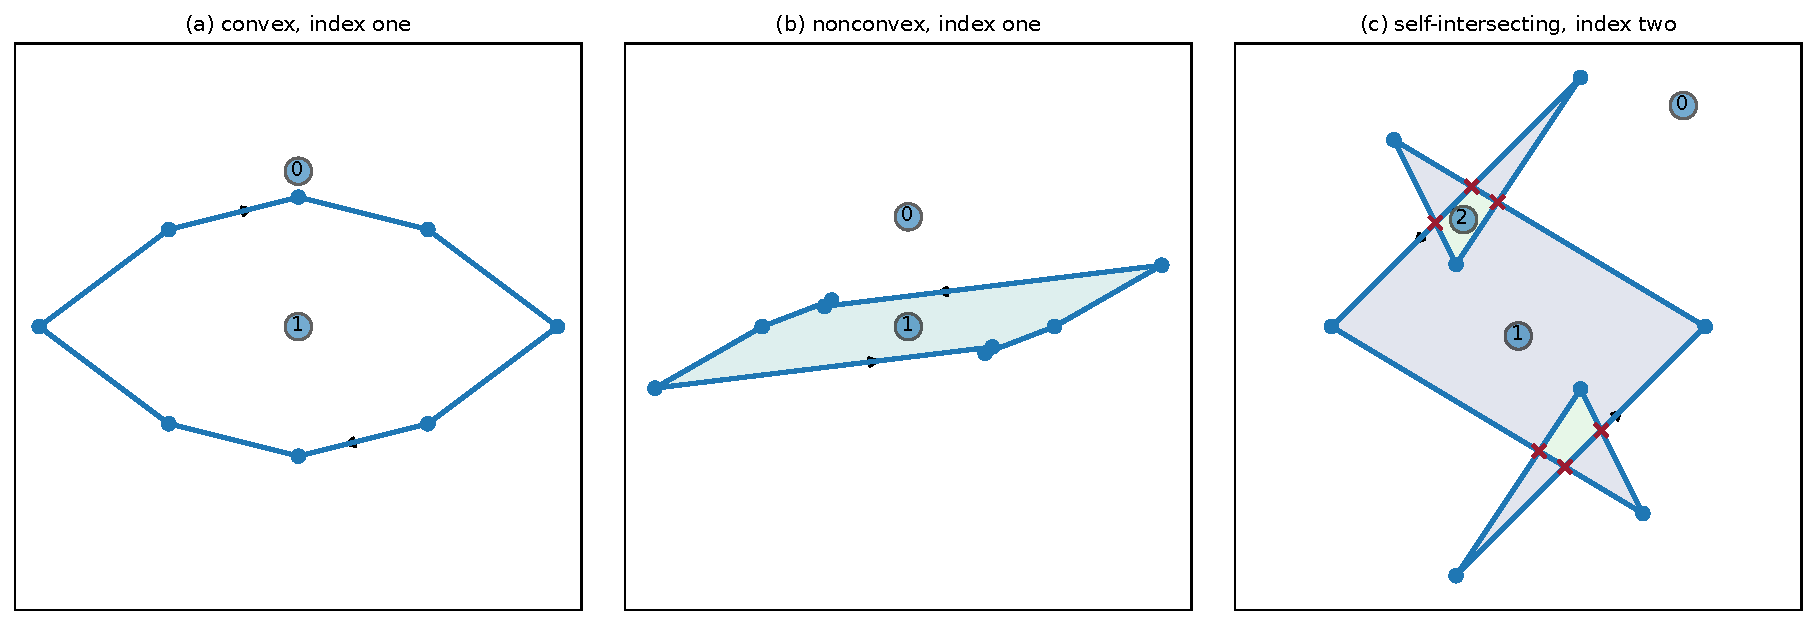
\includegraphics[width=\textwidth]{figures/polygon_regimes.pdf}
\caption{Three boundary-multiplicity regimes.  A sign-coherent convex polygon has winding spectrum $\{0,1\}$ (left).  The witness is nonconvex but remains an index-one Jordan polygon (center).  The exact four-ridge obstruction loop from \Cref{sec:n4} is self-intersecting and contains index-two regions (right); crosses mark its transverse intersections and arrows indicate orientation.  The figure therefore links the polygon geometry of \Cref{sec:simplicity} to the degree formula of \Cref{sec:winding}.}
\label{fig:regimes}
\end{figure}

\Cref{fig:regimes} shows the three multiplicity regimes---convex index one, nonconvex index one, and self-intersecting index two---that connect the classification to the degree formula. The certificate decides each condition of \Cref{prop:simple} by an exact integer predicate: row independence and vertex distinctness by sign of a rational determinant or difference; edge non-collinearity by the sign of a cross product; and disjointness of two edges by exact orientation tests (a pair of segments meets only if the endpoints of each straddle the line of the other, or an endpoint lies on the other segment). No floating-point value enters any comparison. As a cross-check binding the polygon to the determinant certificate of \Cref{app:det}, the same script recomputes the six Cauchy--Binet products $\det(A_{\{i,j\}})\det(B_{\{i,j\}})$ in exact arithmetic and confirms a single negative one, at $\{2,3\}$, matching the value recorded with the witness.

% =====================================================================
\section{Global injectivity of the witness}\label{sec:injectivity}

\begin{corollary}[global injectivity]\label{cor:injective}
The witness network $F(x)=A\sigma(Bx+c)$ of \Cref{thm:separation} is a global $C^1$ diffeomorphism of $\R^2$ onto the open octagon $D$ bounded by $\Gamma$; in particular $F$ is injective.
\end{corollary}

\begin{proof}
The map $F$ is bounded, since $\sigma$ takes values in $(0,1)^N$ and hence $F(\R^2)\subseteq A[0,1]^N$. It is a $C^1$ local diffeomorphism because $\det DF>0$ everywhere; for the witness this is proved analytically (\Cref{prop:analytic-det}) and separately corroborated by the validated interval certificate (\Cref{app:det}), computed directly from \texttt{data/witness.json}. By \Cref{lem:polygon}, the cluster set satisfies $\clinf(F)\subseteq\Gamma$, and by \Cref{prop:simple} the curve $\Gamma$ is a Jordan curve. \Cref{thm:main} applies.
\end{proof}

\begin{theorem}[an open family of globally injective networks]\label{thm:open-family}
There is an open neighborhood $\mathcal U$ of the witness parameters $(A,B,c)$ in $\R^{2\times4}\times\R^{4\times2}\times\R^4$ such that every $(A',B',c')\in\mathcal U$ defines a bounded sigmoid ridge network
\[
 F_{A',B',c'}(x)=A'\sigma(B'x+c')
\]
that is a global $C^1$ diffeomorphism onto the bounded Jordan domain enclosed by its asymptotic polygon.
\end{theorem}

\begin{proof}
The strict row-order and polygon-simplicity inequalities have positive margins, so \Cref{thm:stability} preserves them on an open parameter neighborhood. For the Jacobian, the certificate in \Cref{app:det} consists of two strict parts. On the fixed compact square $K=[-582,582]^2$, the certified interval lower bounds imply $\min_K\det DF>0$.  Joint continuity of $(A,B,c,x)\mapsto\det DF(x)$ and compactness of $K$ preserve this positivity on a parameter neighborhood.  On the tail, the fixed-radius domination proof has a uniform positive angular margin; its finitely many minor, bias, row-norm, grid, and Lipschitz expressions depend continuously on $(A,B,c)$, so the same strict tail inequalities persist after a small perturbation.  Intersecting the compact, tail, row-order, and polygon neighborhoods gives $\mathcal U$.  The cluster-set inversion theorem then applies to every member of $\mathcal U$.
\end{proof}

\begin{corollary}[explicit joint parameter radius]\label{cor:family-radius}
Let $(A_0,B_0,c_0)$ denote the witness parameters.  If
\[
 \max\{\norm{A-A_0}_\infty,\norm{B-B_0}_\infty,
          \norm{c-c_0}_\infty\}\le 5\times10^{-6},
\]
where the matrix norms are entrywise maxima, then the corresponding sigmoid ridge network is a global $C^1$ diffeomorphism onto the bounded Jordan domain enclosed by its asymptotic polygon.
\end{corollary}

\begin{proof}
The exact polygon margins, the compact parameter cover, and the tail-transfer bounds remain strict on the stated cube.  The complete universal enclosure and partition checks are given in \Cref{app:det}; applying \Cref{thm:radius-procedure,thm:main} gives the result.
\end{proof}

A larger anisotropic parameter box is certified in \Cref{cor:anisotropic} in \Cref{app:det}.

\begin{remark}[what is not claimed]\label{rmk:notclaimed}
For the witness result above we do not use any equivalence between simplicity of $\Gamma$ and injectivity; \Cref{sec:winding} establishes the degree--winding criterion by a separate argument.  That criterion does not say that positive Jacobian determinant forces simplicity; it reduces that broader question to the compatibility between local positivity and boundary winding. The present witness lies in the index-one regime.
\end{remark}

% =====================================================================
\section{Planar degree and winding multiplicity}\label{sec:winding}
The inversion theorem of \Cref{sec:theorem} is sufficient but not evidently necessary.  For planar ridge maps, a direct uniform reparameterization of large circles recovers the entire ordered polygonal loop, including the wall edges. This supplies an exact Brouwer-degree count without requiring a separate abstract compactification.

\begin{lemma}[cluster equality under continuous saturation]\label{lem:equality}
Assume the rows are pairwise nonparallel and the activation $f$ is continuous, strictly increasing, and has limits $0$ and $1$.  Then $\clinf(F)=|\gamma|$.
\end{lemma}
\begin{proof}
The inclusion from left to right is the limiting-direction argument of \Cref{lem:polygon}.  Continuity and strict monotonicity make $f$ a homeomorphism from $\R$ onto $(0,1)$.  A vertex is attained along a ray in the corresponding open direction sector.  For an edge point with activation coordinate $t\in(0,1)$ on the wall of row $j$, choose the unique $\tau$ with $f(\tau)=t$, a wall direction $u_j$, and a fixed vector $v_j$ with $b_j\cdot v_j=1$. Then
\[
 x_k=r_k u_j+(\tau-c_j)v_j,\qquad r_k\longrightarrow\infty,
\]
keeps the $j$th logit equal to $\tau$, while every other logit tends to its sector-determined signed infinity.  The edge endpoints follow by saturation. Thus every point of every edge belongs to the cluster set.
\end{proof}

\begin{lemma}[uniform boundary-loop approximation]\label{lem:uniform-loop}
Let
\[
 F(x)=A f(Bx+c):\R^2\longrightarrow\R^2,
\]
where the nonzero rows of $B$ are pairwise nonparallel and $f$ is continuous, strictly increasing, with limits $0$ and $1$.  Let $\gamma:S^1\to\R^2$ be the row-ordered signed-column polygonal loop.  There are orientation-preserving circle homeomorphisms $h_R:S^1\to S^1$ such that
\[
 \sup_{\theta\in S^1}
 \bigl\|F(Ru(h_R(\theta)))-\gamma(\theta)\bigr\|\longrightarrow0,
 \qquad u(\theta)=(\cos\theta,\sin\theta).
\]
\end{lemma}
\begin{proof}
List the $2N$ wall angles cyclically as $\theta_k$.  At the $k$th wall, belonging to row $j(k)$, put
\[
 \varepsilon_k=\sgn\!\bigl(b_{j(k)}\cdot u'(\theta_k)\bigr)\in\{-1,1\}.
\]
Choose an abstract decomposition of $S^1$ into alternating wall intervals $I_k$ and sector intervals $J_k$.  On $J_k$ the loop $\gamma$ is the corresponding saturation vertex.  If $q\in[0,1]$ is the increasing coordinate on $I_k$, then $\gamma$ traverses the signed edge $\varepsilon_k a_{j(k)}$; equivalently, the $j(k)$th target activation coordinate is
\[
 p_k(q)=\begin{cases}q,&\varepsilon_k=1,\\1-q,&\varepsilon_k=-1.\end{cases}
\]

Set $\eta_R=R^{-1/2}$ and let $W_{k,R}=[\theta_k-\eta_R,\theta_k+\eta_R]$.  For all sufficiently large $R$ these windows are disjoint.  The function
\[
 \tau_{k,R}(\theta)=R\,b_{j(k)}\cdot u(\theta)+c_{j(k)}
\]
is strictly monotone on $W_{k,R}$ with sign $\varepsilon_k$, because its derivative divided by $R$ converges uniformly there to $b_{j(k)}\cdot u'(\theta_k)$, and $\lvert b_{j(k)}\cdot u'(\theta_k)\rvert=\norm{b_{j(k)}}\ge\beta:=\min_j\norm{b_j}>0$. A uniform Taylor expansion over the finitely many walls gives
\[
 \tau_{k,R}(\theta_k\pm\eta_R)=c_{j(k)}\pm\varepsilon_k\norm{b_{j(k)}}R^{1/2}+O(1).
\]
Hence, taking $T_R=R^{1/4}$, for all sufficiently large $R$ the interval $[-T_R,T_R]$ lies in the \emph{interior} of every wall-window range, with slack $\beta R^{1/2}-R^{1/4}-O(1)\to\infty$.

Write $g=f^{-1}:(0,1)\to\R$.  On the central part of $I_k$ for which $g(p_k(q))\in[-T_R,T_R]$, define $h_R(q)=\tau_{k,R}^{-1}\bigl(g(p_k(q))\bigr)$; although both $\tau_{k,R}$ and $g\circ p_k$ are decreasing when $\varepsilon_k=-1$, the composition is strictly increasing in $q$ in either case.  On each of the two remaining endpoint pieces extend $h_R$ by a strictly increasing affine homeomorphism onto the corresponding residual subinterval of $W_{k,R}$, nonempty by the strict slack above; map every sector interval $J_k$ by a strictly increasing affine homeomorphism onto the angular sector between its two adjacent wall windows. The endpoint values agree at every seam and the images tile $S^1$ in cyclic order, so the pieces join to an orientation-preserving circle homeomorphism.

On a sector image every wall is at circular distance at least $\eta_R$.  Writing $d_i(\theta)$ for the distance to the wall of row $i$, we have $\lvert b_i\cdot u(\theta)\rvert=\norm{b_i}\,\lvert\sin d_i(\theta)\rvert$, and $\lvert\sin s\rvert\ge 2s/\pi$ on $[0,\pi/2]$ yields a constant $c>0$, independent of $R$, the sector, and $i$, with $\lvert b_i\cdot u(\theta)\rvert\ge c\eta_R$.  Hence every logit satisfies $\lvert R\,b_i\cdot u(\theta)+c_i\rvert\ge cR\eta_R-\lvert c_i\rvert\to\infty$ uniformly, and the activation vector converges to the sector saturation vector. Within $W_{k,R}$, all logits except the $j(k)$th have the same uniform saturation property, since the rows are pairwise nonparallel. On the central wall piece the remaining activation equals $p_k(q)$ exactly.  On the two truncated pieces both the actual and target coordinates lie within
\[
 \delta_R=\max\{f(-T_R),1-f(T_R)\}\longrightarrow0
\]
of the same endpoint value.  Thus the full activation vector converges uniformly to the vertex-or-edge parameterization defining $\gamma$.  Multiplication by the fixed matrix $A$ preserves uniform convergence.
\end{proof}

\begin{theorem}[degree--winding formula]\label{thm:winding}
Under the hypotheses of \Cref{lem:uniform-loop}, suppose in addition that $F$ is $C^1$ and $\det DF$ never vanishes.  Let $\varepsilon=\sgn(\det DF)$.  For every $y\notin|\gamma|$,
\[
 \#F^{-1}(y)=\varepsilon\,\wind(\gamma,y).
\]
\end{theorem}
\begin{proof}
By \Cref{lem:polygon}, $\clinf(F)\subseteq|\gamma|$, so an unbounded sequence of preimages of $y$ would give $y\in\clinf(F)\subseteq|\gamma|$, contrary to $y\notin|\gamma|$.  Thus $F^{-1}(y)$ is compact; local invertibility makes it discrete and therefore finite.  Choose $R$ containing every preimage.  By \Cref{lem:uniform-loop} and the positive distance from $y$ to $|\gamma|$, for all sufficiently large $R$ the loop $F(Ru(h_R(\cdot)))$ is joined to $\gamma$ by the straight-line homotopy in $\R^2\setminus\{y\}$.  Since $h_R$ preserves orientation, this loop has the same winding number as $F|_{\partial B_R}$. Brouwer degree~\cite{outerelo-ruiz} gives
\[
 \deg(F,B_R,y)=\wind(\gamma,y).
\]
Every local degree equals $\varepsilon$, so the left side is $\varepsilon\#F^{-1}(y)$.
\end{proof}

\begin{corollary}[image and multiplicity stratification]\label{cor:image-strata}
Under the hypotheses of \Cref{thm:winding},
\[
 F(\R^2)\setminus|\gamma|
 =\{y\notin|\gamma|:\varepsilon\wind(\gamma,y)>0\}.
\]
On each connected component of $\R^2\setminus|\gamma|$, the number of preimages is constant and equals $\varepsilon\wind(\gamma,y)$.
\end{corollary}
\begin{proof}
The winding number is constant on every complementary component.  By \Cref{thm:winding}, its signed value is exactly the nonnegative integer $\#F^{-1}(y)$, which is positive precisely on the image away from the boundary loop.
\end{proof}

\begin{corollary}[necessary and sufficient planar criterion]\label{cor:iff}
Under the hypotheses of \Cref{thm:winding},
\[
 F\text{ is injective}\iff
 \varepsilon\wind(\gamma,y)\in\{0,1\}
 \quad\text{for every }y\notin|\gamma|.
\]
\end{corollary}
\begin{proof}
The forward implication follows from \Cref{thm:winding}.  Conversely, the formula gives at most one preimage away from the polygonal loop.  If a point of the loop had two finite preimages, inverse-function neighborhoods of those preimages would share a common open image.  Since a polygonal loop has empty interior, that open set contains a nearby point off the loop with two preimages, a contradiction.
\end{proof}

Call the loop \emph{generic} if it has finitely many self-intersections, each a transverse crossing of two edge interiors with no three edges concurrent.  Put $m(y)=\varepsilon\wind(\gamma,y)$, the signed multiplicity from \Cref{thm:winding}; thus $m$ is a nonnegative integer on every complementary region.  Near a transverse crossing, crossing either strand changes $m$ by $\pm1$, so the four local regions carry $m$, $m+a$, $m+b$ and $m+a+b$ for some $a,b\in\{\pm1\}$.  If $a=b=-1$ then nonnegativity forces $m\ge2$; if $a$ and $b$ differ then nonnegativity forces $m\ge1$, and one of $m+a,m+b$ equals $m+1\ge2$; if $a=b=+1$ then $m+a+b=m+2\ge2$.  Thus every generic self-crossing creates a region of multiplicity at least two. Hence, in the generic class, $F$ is injective if and only if its asymptotic polygon is simple.  The exact signed-multiplicity spectra are computed by \path{code/polygon_winding.py}: the witness octagon has spectrum $\{0,1\}$, and an exact self-intersecting centrally symmetric example has spectrum $\{0,1,2\}$ (\path{results/structural/winding_spectra.json}).

% =====================================================================
\section{The remaining four-ridge boundary obstruction}\label{sec:n4}
For $n=2$, $N=4$, the boundary loop is a centrally symmetric octagon. \Cref{cor:iff} makes its signed winding spectrum the exact multiplicity invariant. The witness studied here has spectrum $\{0,1\}$ and is injective. More generally, the degree--winding formula shows that a positive-Jacobian network would fail to be injective precisely when its asymptotic octagon has a region of winding at least two. Thus the unrestricted four-ridge question is reduced to compatibility between pointwise determinant positivity and such boundary winding.  That compatibility question lies outside the scope of the present paper; none of the results proved here depends on its resolution.

Central symmetry by itself does not control the spectrum.  For comparison, the exact loop with first-half edges
\[
 (2,3),\quad(-4,-4),\quad(5,-3),\quad(-1,2)
\]
has winding spectrum $\{0,1,2\}$.  A ridge realization of that loop was constructed and has $\det DF\approx-0.186$ at $(-\tfrac{11}{10},-\tfrac{57}{20})$, so this auxiliary loop does not itself satisfy the positive-Jacobian hypothesis.  The exact regression probe is implemented in
\begin{center}
\small\path{code/probe_n4_winding_obstruction.py}.
\end{center}

% =====================================================================
\section{Novelty and relation to existing methods}\label{sec:novelty}

The theorem package has several layers of different novelty.  The covering-space argument in \Cref{thm:main} is a compact specialization of classical proper-local-homeomorphism and Hadamard-type global inversion \cite{gutu-jaramillo,ruzhansky-sugimoto}, with the cluster boundary supplying both relative properness and identification of the image; it should not be presented as a new branch of topology.  The cluster-polygon lemma is elementary once the row arrangement is written down.  Likewise, the all-cases orientation formula in \Cref{thm:closed-form} specializes standard exact segment-intersection predicates from computational geometry~\cite{deberg}.

The paper's substantive contribution is their assembly for bounded ridge maps and the geometry exposed by that assembly.  In particular, \Cref{thm:mixed-convexity} turns the sign-coherent maximal-minor regime studied in \cite{mhr,fmr} into a concrete boundary statement: it is exactly the regime in which the asymptotic polygon is strictly convex.  The witness lies immediately outside that regime, and \Cref{prop:sign-insufficient,thm:one-sided,thm:graph-gap} show why a magnitude-sensitive refinement is required and how one can certify it. The analytic class in \Cref{cor:analytic-class} is independent of the spatial branch-and-bound, while the explicit quantitative boxes in \Cref{thm:open-family,cor:family-radius} use the strict validated determinant certificate. Together they are stronger than a single computer-checked example.

The adjacent neural-injectivity literature includes global characterizations for ReLU networks and related injective architectures~\cite{puthawala}.  Sign-vector and maximal-minor criteria for generalized polynomial and monotone map families are developed in~\cite{muller-sign,mhr,fmr}, while classical zonotope theory explains why angularly ordered generators bound a convex zonogon~\cite{ziegler}. Those sources cover the convex/sign-coherent side of the picture.  A targeted literature search for this revision located no prior result that (a) identifies a bounded saturating ridge map's cluster set at infinity exactly with its row-ordered signed-column polygonal loop, (b) separates mixed-minor convexity from magnitude-sensitive simplicity, and (c) combines that geometry with a quantitative global-injectivity neighborhood.  This supports novelty of the package, not absolute priority; the individual segment predicates, covering-space facts, and zonogon boundary order remain classical ingredients.

The degree--winding result adds a different layer: after a uniform reparameterization of large circles, the asymptotic loop becomes a complete multiplicity invariant off its image, not merely a sufficient Jordan-boundary certificate.  The derivative-weight formulation likewise isolates the precise convexification gap behind the separation: $Q_M$ is positive on the nonlinear weight image but negative at a path barycenter.  These two statements---exact boundary multiplicity and interior weight convexification---are the principal conceptual advances of the unified manuscript.

% =====================================================================
\section{Derivative-weight geometry and the failure of mean-value univalence}\label{sec:reconcile}

\Cref{prop:weight-average} gives the precise geometry behind the separation. The pointwise Jacobian condition is
\[
 Q_M(w)>0\qquad\text{for every }w\in\Wder,
\]
whereas the segment-averaged certificate evaluates the same indefinite quadratic form at a path barycenter
\[
 \bar w=\int_0^1\sigma'\bigl(B(p+t(q-p))+c\bigr)\,dt
 \in\operatorname{conv}(\Wder).
\]
For the witness, $Q_M$ is positive on the entire derivative-weight image but $Q_M(\bar w)<0$ at the explicit pair $(p,q)$.  The weighted-AM--GM argument in \Cref{sec:weights} explains why the nonlinear image stays on the positive side of the quadratic zero cone; averaging need not preserve that constraint and can cross the cone.

Numerically,
\[
\overline{DF}(p,q)\approx
\begin{pmatrix} \phantom{-}0.14765107 & -0.08252810\\
                \phantom{-}0.22828004 & -0.12771136 \end{pmatrix},
\quad \sigma_{\min}\approx 5.52\times10^{-5},\quad
\kappa_2\approx 5.64\times10^{3};
\]
its determinant is approximately $-1.71998\times10^{-5}$, computed from the unrounded entries.  At the coincident pair, $\overline{DF}(p,p)=DF(p)$ has positive determinant.  Continuity along the endpoint therefore yields an intermediate pair at which the averaged Jacobian is exactly singular.  The mean-value hypothesis does not merely become weak or ill-conditioned; it fails outright.

This does not conflict with \Cref{cor:injective}.  Local orientation is governed by $Q_M$ on $\Wder$, while global multiplicity is governed by the winding of the asymptotic tope-cycle polygon.  The witness has winding spectrum $\{0,1\}$ and is therefore one-sheeted even though a derivative-weight barycenter defeats the mean-value certificate.  The two tests probe different geometries.

% =====================================================================
\section{Conclusion: interior weights and boundary degree}\label{sec:conclusion}

The paper identifies an interior--boundary factorization for planar bounded ridge maps.  The derivative-weight image and its mixed-minor quadratic form control local orientation; the asymptotic polygon and its winding function control the complete sheet structure away from the cluster boundary.  In oriented-matroid language, topes produce the boundary cycle, chirotopes identify the convex sign-coherent regime, and a row circuit supplies the analytic determinant dominance mechanism.

For the canonical network these pieces close the full separation story: the Jacobian is analytically positive, the asymptotic polygon is a nonconvex Jordan octagon of index one, and the map is a global diffeomorphism, although a segment average crosses the quadratic zero cone. Thus averaged-Jacobian nonsingularity is not necessary for injectivity, while the asymptotic loop determines the exact sheet number once local orientation is fixed.

% =====================================================================
\section{Verification and reproducibility}\label{sec:verification}

\paragraph{Artifact of record.} The source, exact witness data, figures,
configuration files, certificate and replay scripts, and machine-readable
reports are archived at
\href{https://github.com/lmdixon23/njc-2026-cluster-inversion}{github.com/lmdixon23/njc-2026-cluster-inversion},
release tag \texttt{v1.2.0}. The public claim map and verification guide are
\path{verification/CLAIM-TO-ARTIFACT-MAP.md} and
\path{verification/README.md}.

\paragraph{Claim-to-artifact map.} \Cref{tab:artifacts} maps each load-bearing
claim to its primary evidence and its separate check or failure condition.

\begin{table}[H]
\centering\small
\begin{tabular}{@{}>{\raggedright\arraybackslash}p{0.29\textwidth}>{\raggedright\arraybackslash}p{0.25\textwidth}>{\raggedright\arraybackslash}p{0.36\textwidth}@{}}
\toprule
Claim & Primary evidence & Separate check or failure condition\\
\midrule
Cluster-boundary inversion & Proof of \Cref{thm:main} & Direct check of every topological hypothesis\\
Asymptotic polygon and classification &
Proofs and exact rational geometry &
Complete segment formula and three-regime examples\\
Witness polygon & Seven rational signs & All 20 nonadjacent pairs checked exactly\\
Pointwise $\det DF>0$ (witness) &
Analytic weighted-AM--GM proof, \Cref{prop:analytic-det} &
Validated compact/tail certificate (\Cref{app:det})\\
Common radius $5\times10^{-6}$ &
Interval certificate: 93,000 leaves &
Exact tiling replay; Decimal diagnostic; complete Arb leaf replay\\
Degree--winding formula &
Uniform boundary-loop lemma and Brouwer degree &
Separate proof reconstruction; three exact-arithmetic spectrum implementations\\
Separation from averaged Jacobian &
Validated interval certificate, \path{code/certify_avgdet_neg.py} &
Closed-form high-precision recomputation and IVT argument\\
\bottomrule
\end{tabular}
\caption{Claim-to-artifact map. The maintained release gate validates report semantics and bindings in addition to file hashes. Its focused negative tests require nonzero exits for ambiguous intervals, incomplete coverage, exhausted budgets, forged checkpoints, contradictory reports, and omitted manifest entries.}
\label{tab:artifacts}
\end{table}

\paragraph{Reproduction protocol.} From the repository root, the maintained
release gate is
\begin{quote}\ttfamily bash run\_all.sh
\end{quote}
The gate must run under the interpreter that carries \texttt{requirements-lock.txt}.  The script selects one that can import \texttt{python-flint} and prints it before the first check; an explicit choice may be supplied as \texttt{PY=/path/to/python bash run\_all.sh}.  On systems where \texttt{bash} resolves to the Windows Subsystem for Linux, the default interpreter is a separate installation and may lack those dependencies even when a native installation carries them.  The repository fixes LF line endings on every platform through \texttt{.gitattributes}, and the artifact writers pin LF explicitly; a manifest mismatch accompanied by a clean \texttt{git status} therefore indicates a line-ending translation rather than a content difference.  Persisted certificate reports carry no wall-clock timings, so re-running any certification reproduces its artifacts byte for byte and the manifest remains valid.  All script output is ASCII, so the gate may be run with its output redirected to a file or captured by a continuous-integration job on any platform.
and ends with \texttt{VERDICT: ALL MAINTAINED CHECKS PASSED}. The expensive
common-radius workflow is
\begin{quote}\ttfamily python code/certify\_open\_family.py config/witness\_common.json.
\end{quote}
Using \path{config/witness_anisotropic.json} instead selects the larger
anisotropic box. Compact leaves are exported as binary split paths.
The Decimal replay reconstructs them from the root and proves prefix-freeness
and exact dyadic volume closure; its determinant reevaluation is a
corroborating numerical diagnostic. Separately, the Arb compact replay
reconstructs and rigorously rescores every exported leaf using ball arithmetic,
and the Arb tail replay rescores all $200{,}000$ fixed-radius angular directions.
A separate tail-transfer checker rederives the minor and
logarithmic loss bounds. Each combined parameter report
embeds the SHA-256 and byte count of every subreport it summarizes; the verifier
recomputes the semantic verdicts, checks the exact expected component set, and
rejects stale or mismatched configuration, witness, report, and leaf bindings.

\paragraph{Analytic and degree checks.} \texttt{bash code/run\_structural\_checks.sh} runs the scalar analytic-determinant certificate, the exact winding-spectrum computation, and the four-ridge winding-two probe, each fail-closed (\Cref{sec:weights,sec:winding,sec:n4}). The witness spectrum $\{0,1\}$ was confirmed by three exact-arithmetic implementations, including a separate SymPy kernel.

\paragraph{Quantitative records.} For the common cube the interval workflow processed $185{,}999$ boxes and certified $93{,}000$ terminal leaves; the separate Arb replay checked all $93{,}000$, with minimum replayed lower endpoint approximately $2.04\times10^{-248}$.  For the anisotropic box the workflow processed $193{,}033$ boxes and certified $96{,}517$ leaves; the replay checked all leaves and exact volume closure.  The point-tail grid was recomputed in this package and has rigorous recorded margin $0.0273200022\ldots$, justifying the conservative base value $0.0273$.

\paragraph{Falsification criteria.} The geometry checker rejects row dependence, repeated vertices, zero edges, adjacent overlap, or any nonadjacent intersection.  Parameter certificates reject ambiguous minor signs, any compact leaf whose determinant lower endpoint is not strictly positive, incomplete partition volume, a non-prefix-free path set, or a nonpositive tail residual. The package verifier also rejects missing expected reports or content-hash mismatches.

\paragraph{Limitations.} The exact simplicity formula is semialgebraic rather than sign-only; \Cref{prop:sign-insufficient} proves that sign-only data cannot suffice outside the convex regime. The radii are conservative inner bounds and are not maximal. The generating compact certificates use \texttt{mpmath.iv} 1.3.0, whose \href{https://mpmath.org/doc/current/contexts.html}{official documentation} states interval-containment semantics while designating the interval subsystem experimental. The public Arb implementation therefore reconstructs and rigorously rescores every exported leaf; the separate Decimal layer is retained for partition reconstruction and diagnostic rescoring. The polygon method is planar and assumes bounded saturating activations with a nondegenerate row arrangement. The degree argument assumes a continuous strictly increasing saturating activation and pairwise nonparallel rows; the equivalence between injectivity and polygon simplicity is stated only in generic transverse position. The degree--winding chain has been separately reconstructed, and the witness spectrum has been checked in three exact-arithmetic kernels. These verification records do not substitute for journal peer review.

% =====================================================================
\section*{Declarations}
\paragraph{Funding.} No funding was received for this work.
\paragraph{Competing interests.} The author declares no competing interests.
\paragraph{Data and code availability.} Code, data, certificates, and
verification materials are available at
\href{https://github.com/lmdixon23/njc-2026-cluster-inversion}{github.com/lmdixon23/njc-2026-cluster-inversion},
release tag \texttt{v1.2.0}. The repository contains the exact witness,
scripts, configuration files, and machine-readable results used in the paper.
\paragraph{AI assistance.} Text-to-text generative AI tools, including Claude and GPT, assisted with candidate exploration, code drafting and review, adversarial checking, and editorial revision. Any AI-assisted mathematical claim, source attribution, code fragment, constant, or numerical output retained in the work was checked separately from the originating AI response through hand derivation, source verification, exact recomputation, or validated numerical computation as appropriate. The author determined the research direction and acceptance criteria and assumes full responsibility for the work.

% =====================================================================
\appendix
\section{Proofs of the cluster-set inversion theorem and the ridge cluster lemma}\label{app:proof}

We use four standard facts, each with its hypotheses met in the application.
\begin{enumerate}[label=(T\arabic*),leftmargin=*]
\item \emph{Jordan curve theorem.} A Jordan curve $\Gamma\subset\R^2$ separates $\R^2\setminus\Gamma$ into two connected open sets, one bounded ($D$) and one unbounded ($E$), with $\Gamma=\partial D=\partial E$~\cite{thomassen}.
\item \emph{Jordan--Schoenflies theorem (planar).} Every Jordan curve extends to a self-homeomorphism of $\R^2$ carrying $\Gamma$ to the unit circle; hence $D$ is homeomorphic to an open disk, in particular simply connected and locally path-connected~\cite{thomassen}.
\item \emph{Properness and closedness.} A continuous proper map into a locally compact Hausdorff space is closed~\cite{ho}.
\item \emph{Proper local homeomorphisms are coverings.} A proper local homeomorphism from a Hausdorff space onto a locally compact, locally connected Hausdorff space is a covering map~\cite{ho}.
\end{enumerate}
Throughout, $\clinf(F)$ is closed, being the nested intersection $\bigcap_{R>0}\overline{F(\{\norm{x}>R\})}$ of closed sets; when $F$ is bounded it is nonempty and compact, so the hypothesis $\clinf(F)\subseteq\Gamma$ is not vacuous.

\begin{proof}[Proof of \Cref{thm:main}]
Let $E$ be the unbounded component of $\R^2\setminus\Gamma$.

\emph{Step A (relative properness).} Let $K\subseteq\R^2\setminus\Gamma$ be compact. The preimage $F^{-1}(K)$ is closed by continuity, and it is bounded: otherwise there are $x_k\in F^{-1}(K)$ with $\norm{x_k}\to\infty$, and, $K$ being compact, a subsequence of $F(x_k)$ converges to some $y\in K$; then $y\in\clinf(F)\subseteq\Gamma$, so $y\in K\cap\Gamma=\varnothing$, a contradiction. A closed bounded subset of $\R^2$ is compact, so $F^{-1}(K)$ is compact.

\emph{Step B (the image misses $E$).} Put $P:=F^{-1}(E)$, an open set. The restriction $F|_P\colon P\to E$ is open, being a local homeomorphism restricted to an open set. It is proper: for compact $K\subseteq E$ one has $K\subseteq\R^2\setminus\Gamma$, so $F^{-1}(K)$ is compact by Step~A, and $K\subseteq E$ gives $F^{-1}(K)\subseteq P$, whence $(F|_P)^{-1}(K)=F^{-1}(K)$ is compact. By (T3) with the locally compact Hausdorff target $E$, the map $F|_P$ is closed. Thus $F(P)$ is open and closed in the connected set $E$; were it nonempty it would equal $E$, impossible because $F(\R^2)$ is bounded while $E$ is not. Hence $P=\varnothing$, that is, $F(\R^2)\cap E=\varnothing$. (Connectedness of $P$ is not used: openness is pointwise, closedness is properness of the whole restriction, and the conclusion is drawn in the connected target $E$.)

\emph{Step C (the image misses $\Gamma$).} Suppose $F(x_0)\in\Gamma$. As a local homeomorphism $F$ is open at $x_0$, so some open neighborhood $U$ of $F(x_0)$ lies in $F(\R^2)$. By (T1), $\Gamma=\partial E$, so $F(x_0)$ is a limit of points of $E$ and $U\cap E\neq\varnothing$; then $F(\R^2)\cap E\neq\varnothing$, contradicting Step~B. Therefore $F(\R^2)\cap\Gamma=\varnothing$, and with Step~B one has $F(\R^2)\subseteq D$.

\emph{Step D (surjectivity onto $D$).} View $F$ as a map $\R^2\to D$, well defined by Step~C. It is proper: a compact $K\subseteq D$ is disjoint from $\Gamma$, so $K\subseteq\R^2\setminus\Gamma$ and $F^{-1}(K)$ is compact by Step~A. The image $F(\R^2)$ is open (local homeomorphism) and closed in $D$ (properness with (T3)); a nonempty open-and-closed subset of the connected set $D$ is all of $D$.

\emph{Step E (a single sheet).} By Steps~A--D, $F\colon\R^2\to D$ is a proper surjective local homeomorphism onto $D$, an open subset of $\R^2$ and hence locally compact, locally connected, and Hausdorff. By (T4), $F$ is a covering map. By (T2), $D$ is simply connected and locally path-connected; a covering of such a space with connected total space $\R^2$ has a single sheet, so $F$ is a homeomorphism of $\R^2$ onto $D$. If in addition $F$ is $C^1$ with $\det DF\neq0$ everywhere, the inverse function theorem furnishes local $C^1$ inverses, which coincide with the inverse of the bijection $F$; hence $F$ is a $C^1$ diffeomorphism.
\end{proof}

\begin{proof}[Proof of \Cref{lem:polygon}]
Let $x_k$ satisfy $\norm{x_k}\to\infty$ and $F(x_k)\to y$; we show $y\in\Gamma$. Passing to a subsequence, $u_k:=x_k/\norm{x_k}\to u\in S^1$. Fix an index $i$ with $b_i\cdot u\neq0$. Then $b_i\cdot x_k+c_i=\norm{x_k}\,(b_i\cdot u_k)+c_i$ tends to $+\infty$ if $b_i\cdot u>0$ and to $-\infty$ if $b_i\cdot u<0$, so $f(b_i\cdot x_k+c_i)\to 1$ or $0$ accordingly, by the endpoint limits of $f$. At most one index $j$ has $b_j\cdot u=0$: two rows orthogonal to the nonzero vector $u$ would be parallel, against the hypothesis. For that exceptional $j$, if it occurs, the value $f(b_j\cdot x_k+c_j)$ lies in $[0,1]$; pass to a further subsequence converging to some $t\in[0,1]$. With $S=\{\,i:b_i\cdot u>0\,\}$, continuity of $y\mapsto Ay$ gives
\[
F(x_k)\longrightarrow \sum_{i\in S} a_i + t\,a_j = V(S)+t\,a_j,
\]
a point on the closed edge of $\Gamma$ from $V(S)$ to $V(S\cup\{j\})$ (and the vertex $V(S)$ itself when no such $j$ occurs). Hence $y\in\Gamma$. Only the monotonicity and the two endpoint limits of $f$ entered the argument.
\end{proof}

\section{Complete polygon predicates}\label{app:polygon-criteria}

The main text uses structural criteria that expose the geometry.  For completeness, this appendix records the exact all-cases predicate and the graph-gap specialization.

For an all-cases algebraic formulation, write the cyclic vertices as $v_0,\ldots,v_{2N-1}$ and $E_r=[v_r,v_{r+1}]$, with indices modulo $2N$. For points $x,p,q\in\R^2$, define
\[
 \operatorname{On}(x;p,q)
 \iff
 \det(q-p,x-p)=0,
 \quad
 (x_j-p_j)(x_j-q_j)\le0\quad(j=1,2).
\]
For two edges put
\[
 \omega_1=\det(v_{r+1}-v_r,v_s-v_r),\quad
 \omega_2=\det(v_{r+1}-v_r,v_{s+1}-v_r),
\]
\[
 \omega_3=\det(v_{s+1}-v_s,v_r-v_s),\quad
 \omega_4=\det(v_{s+1}-v_s,v_{r+1}-v_s),
\]
and let $\operatorname{Meet}(r,s)$ be the Boolean formula
\[
 (\omega_1\omega_2<0\ \wedge\ \omega_3\omega_4<0)
 \ \vee\
 \bigvee_{x\in\{v_s,v_{s+1}\}}\operatorname{On}(x;v_r,v_{r+1})
 \ \vee\
 \bigvee_{x\in\{v_r,v_{r+1}\}}\operatorname{On}(x;v_s,v_{s+1}).
\]

\begin{theorem}[closed sign-plus-magnitude formula]\label{thm:closed-form}
For a fixed row order and switch signs, the asymptotic polygon is simple if and only if:
\begin{enumerate}[label=(\roman*),leftmargin=*]
\item all cyclic vertices are distinct and every edge is nonzero;
\item adjacent edges meet only at their shared endpoint; equivalently, for every consecutive triple $(v_{r-1},v_r,v_{r+1})$, neither outer vertex lies on the other adjacent edge;
\item $\neg\operatorname{Meet}(r,s)$ for every nonadjacent pair of edges.
\end{enumerate}
Every quantity in this formula is a polynomial in the entries of $A$ once the cyclic order supplied by $B$ is fixed.  Thus the simple-polygon locus is an open semialgebraic subset of each nondegenerate row-order chamber.
\end{theorem}

\begin{proof}
The formula is the exact orientation test for two closed line segments, including collinear endpoint and overlap cases.  Conditions (i)--(ii) make the cyclic piecewise-linear parametrization locally embedded at its vertices; condition (iii) excludes every other self-intersection.  Conversely, every failure of simplicity is either a repeated/zero local feature, an adjacent overlap, or an intersection of nonadjacent edges.  Since each $v_r$ is a signed partial sum of columns of $A$, the orientation and coordinate-order predicates are polynomial inequalities in those entries.
\end{proof}

The one-sided condition is sufficient rather than necessary.  A complete formula within the common-half-plane class follows by representing the two chains as graphs.

\begin{theorem}[monotone graph-gap criterion]\label{thm:graph-gap}
Assume $q(g_k)>0$ for every $k$, choose a linear functional $r$ independent of $q$, and put
\[
 x_k=q(p_k),\quad y_k=r(p_k),\quad T=q(S),\quad Y=r(S).
\]
Let $f:[0,T]\to\R$ be the piecewise-linear graph through $(x_k,y_k)$ and define
\[
 H(x)=f(x)+f(T-x)-Y.
\]
Then the asymptotic polygon is simple if and only if $H(x)\neq0$ for every $0<x<T$.  If the interior breakpoint set below is nonempty, this is equivalent to requiring one common strict sign at every breakpoint:
\[
 \mathcal B=\{x_k,T-x_k:1\le k<N\}\cap(0,T),
\]
all values $H(\beta)$ have one common strict sign.  If $\mathcal B=\varnothing$, the criterion is the direct condition $H(x)\neq0$ on $(0,T)$; it cannot be replaced by a vacuous finite sign test.
\end{theorem}

\begin{proof}
The first chain is the graph $y=f(x)$ and its reflection is $y=Y-f(T-x)$, so they meet at an interior abscissa exactly when $H(x)=0$. The function $H$ is affine between consecutive points of $\{0,T\}\cup\mathcal B$ and satisfies $H(0)=H(T)=0$.  When $\mathcal B$ is nonempty, it is nonzero on the open interval precisely when all interior breakpoint values have one strict sign.  When $\mathcal B$ is empty, the direct open-interval condition is retained.
\end{proof}

\section{A validated-interval certificate that \texorpdfstring{$\det DF>0$}{det DF>0}}\label{app:det}

\subsection{General robustness-radius procedure}\label{app:radius-procedure}

\begin{theorem}[certified robustness-radius procedure]\label{thm:radius-procedure}
Let $F_{\theta_0}(x)=A_0\sigma(B_0x+c_0)$ be a planar ridge network for which (i) an exact asymptotic-polygon certificate has strict row-order and simplicity margins, (ii) a finite interval cover certifies $\det DF_{\theta_0}>0$ on a compact square $[-R,R]^2$, and (iii) a finite angular certificate proves a strict tail-domination margin outside the radius $R$.  Replace each parameter entry by an interval box of prescribed radius, recompute the polygon inequalities, every compact-cover leaf, every Cauchy--Binet minor interval, and the analytic tail-loss bound.  If all resulting inequalities remain strict, then every parameter in the box defines a global diffeomorphism onto the bounded domain enclosed by its asymptotic polygon.
\end{theorem}

\begin{proof}
The interval tests quantify universally over the parameter box.  The exact polygon inequalities preserve the row chamber and a Jordan asymptotic polygon. The compact leaf cover and tail certificate together prove $\det DF_\theta>0$ on all of $\R^2$ for every enclosed $\theta$.  The ridge cluster-set lemma and \Cref{thm:main} then apply uniformly.  No optimization claim is involved: any box that passes is a certified inner approximation to the open injective locus.
\end{proof}

\begin{remark}
The procedure is implemented by \path{code/certify_open_family.py}.  It accepts a configuration file, exports a prefix-free compact leaf cover, and can invoke a second arithmetic implementation to replay both the compact and tail parts. The current tail module covers the one-negative-minor domination regime; the geometric and compact-cover components accept arbitrary planar hidden width.
\end{remark}

\subsection{Certified parameter boxes}\label{app:quant-boxes}
The common cube stated in \Cref{cor:family-radius} is certified as follows.  The common radius $5\times10^{-6}$ is below the exact polygon-generator and row-arrangement radii.  On $[-582,582]^2$, the parameter-box branch-and-bound certifies all $93{,}000$ leaves with no unresolved leaf or budget exhaustion.  In the tail, the point margin $0.0273200022\ldots$ is conservatively replaced by $0.0273$; the uniform perturbation loss is below $0.016990355$, leaving residual margin above $0.010309645$.  The mixed-minor signs remain fixed throughout the cube.  Hence \Cref{thm:radius-procedure} applies.

\begin{corollary}[an anisotropic parameter box]\label{cor:anisotropic}
The same conclusion holds throughout the entrywise box
\[
 \norm{A-A_0}_\infty\le10^{-4},\qquad
 \norm{B-B_0}_\infty\le3\times10^{-6},\qquad
 \norm{c-c_0}_\infty\le10^{-3}.
\]
\end{corollary}

\begin{proof}
The exact geometry bounds absorb the stated $A$ and $B$ perturbations. The compact parameter cover has $96{,}517$ terminal leaves. The \path{mpmath.iv} interval workflow generates the cover, a separate Arb implementation rigorously rescores every leaf, and a custom Decimal implementation separately reconstructs the prefix-free partition, verifies exact volume closure, and diagnostically rescores every leaf. The tail transfer retains a lower margin exceeding $0.00415$, recomputed in a separate Decimal implementation. Apply \Cref{thm:radius-procedure}.
\end{proof}

\begin{remark}[quantitative certificate]
The generating compact certificates use \texttt{mpmath.iv}. A separately written Arb layer reconstructs every dyadic leaf from its split path and rigorously verifies determinant positivity on the complete common and anisotropic covers. A third Decimal layer verifies prefix-freeness and exact volume closure and retains its determinant reevaluation as a diagnostic cross-check. The maintained verifier binds all three records to the exact witness, configuration, compact report, and leaf export.
\end{remark}

For $F(x)=A\sigma(Bx+c)$ the Cauchy--Binet expansion gives
\[
\det DF(x)=\sum_{\{i,j\}}\det(A_{\{i,j\}})\,\det(B_{\{i,j\}})\;
\sigma'(z_i)\,\sigma'(z_j),\qquad z=Bx+c,
\]
a sum over the six pairs of hidden units, where $A_{\{i,j\}}$ is the $2\times2$ column submatrix of $A$ and $B_{\{i,j\}}$ the $2\times2$ row submatrix of $B$. For the witness exactly one product $m_{ij}:=\det(A_{\{i,j\}})\det(B_{\{i,j\}})$ is negative, at $\{i,j\}=\{2,3\}$; the other five are positive. Positivity of $\det DF$ is therefore a domination statement: the five positive terms must outweigh the single negative one everywhere.

The exact determinant certificate reads $A,B,c$ as exact rationals from the
canonical witness file, with no intermediate pickle. It forms
the six $m_{ij}$ exactly and encloses
$\sigma'(t)=1/(2+e^{t}+e^{-t})$ in interval arithmetic
(\texttt{mpmath.iv}); the denominator exceeds $4$, so the reciprocal is safe.
A box in $x$ is \emph{certified} only when the lower end of the resulting
interval enclosure of $\det DF$ is strictly positive. This is decided by
interval comparison, never a midpoint test, so a reported certification is
rigorous at any working precision; lower precision merely widens enclosures and
forces more subdivision. The run has two parts.
\begin{itemize}[leftmargin=*]
\item \emph{Tail (fixed radius).} We certify a \emph{fixed} radius $R$ directly, rather than a supremum of quotients. For a unit direction $u$ and a positive pair $\{k,l\}$ put $g_{kl}(u)=\rho_2(u)+\rho_3(u)-\rho_k(u)-\rho_l(u)$ with $\rho_i(u)=|b_i\cdot u|$; the pair dominates the negative term at radius $R$ when $g_{kl}(u)>0$ and $R\,g_{kl}(u)>K_{kl}$, where $K_{kl}=\ln\!\bigl(16\,|m_{23}|/m_{kl}\bigr)+|c_2|+|c_3|+|c_k|+|c_l|$ (from $\sum|t_{\{2,3\}}|-\sum|t_{\{k,l\}}|\ge r\,g_{kl}-\sum|c|$ and $\sigma'(t)\in[\tfrac14 e^{-|t|},\,e^{-|t|}]$). For a proposed integer $R$ the certifier checks, at every point of an angular grid, that some positive pair has $g_{kl}>0$ and $R\,g_{kl}-K_{kl}>0$ after subtracting the between-grid Lipschitz allowance $R\,L_{kl}\,\Delta\theta/2$ with $L_{kl}=\norm{b_2}+\norm{b_3}+\norm{b_k}+\norm{b_l}$; the dominating pair may switch between neighboring directions. All bounds are outward, so a positive verdict is rigorous, and the test is monotone in $R$.
\item \emph{Interior.} On $[-R_0,R_0]^2$ an adaptive branch-and-bound certifies each box or bisects it; a box that reaches the resolution floor uncertified, or exhaustion of the search budget, forces a hard failure (nonzero exit).
\end{itemize}
For the witness the fixed-radius test certifies $R_0=582$ (worst-direction margin $\approx 2.7\times10^{-2}$), and the interior branch-and-bound on $[-582,582]^2$ processes $185{,}999$ boxes and certifies all $93{,}000$ terminal boxes, with none left uncertified at the resolution floor and no budget exhaustion, in a few minutes on typical current hardware; hence $\det DF(x)>0$ for all $x\in\R^2$. A self-test validates the $\sigma'$ enclosures against a reference, confirms the exact minor products and their single negative sign, checks that the interval determinant encloses the true value at a sample point, plants an inflated negative term that the checker must refuse, and confirms that the tail certifier rejects a too-small radius.

\begin{remark}[relation between the two positivity proofs]\label{rmk:companion-det}
The analytic argument in \Cref{prop:analytic-det} is the primary proof of $\det DF>0$ for the witness.  The present interval certificate rederives the same conclusion from the exact rational entries of \texttt{witness.json} using a spatial compact--tail decomposition.  It provides separate computational corroboration for the witness and carries the explicit parameter boxes in \Cref{cor:family-radius,cor:anisotropic}.
\end{remark}

% =====================================================================
\begin{sloppypar}
\raggedright
\begin{thebibliography}{99}
\bibitem{chen-jiang} X.~Chen and X.~Jiang, \emph{Moonshine: an autonomous mathematical research agent centered on conjecture generation}, \href{https://arxiv.org/abs/2606.10806}{arXiv:2606.10806}, 2026. (The Neural Jacobian Conjecture studied here is formulated in this work.)
\bibitem{muller-sign} S.~M\"uller, E.~Feliu, G.~Regensburger, C.~Conradi, A.~Shiu, and A.~Dickenstein, \emph{Sign conditions for injectivity of generalized polynomial maps with applications to chemical reaction networks and real algebraic geometry}, Found. Comput. Math. \textbf{16} (2016), 69--97; \href{https://arxiv.org/abs/1311.5493}{arXiv:1311.5493}.
\bibitem{ziegler} G.~M. Ziegler, \emph{Lectures on Polytopes}, Graduate Texts in Mathematics 152, Springer, 1995.
\bibitem{mhr} S.~M\"uller, J.~Hofbauer, and G.~Regensburger, \emph{On the bijectivity of families of exponential/generalized polynomial maps}, SIAM J.\ Appl.\ Algebra Geom.\ \textbf{3} (2019), no.~3, 412--438; \href{https://arxiv.org/abs/1804.01851}{arXiv:1804.01851}.
\bibitem{fmr} E.~Feliu, S.~M\"uller, and G.~Regensburger, \emph{Characterizing injectivity of classes of maps via classes of matrices}, Linear Algebra Appl.\ \textbf{580} (2019), 236--261; \href{https://arxiv.org/abs/1901.11272}{arXiv:1901.11272}.
\bibitem{gutu-jaramillo} O.~Gut\'u and J.~A.~Jaramillo, \emph{Global homeomorphism and covering projections on metric spaces}, \href{https://arxiv.org/abs/math/0606569}{arXiv:math/0606569}, 2006.
\bibitem{ruzhansky-sugimoto} M.~Ruzhansky and M.~Sugimoto, \emph{On global inversion of homogeneous maps}, Bull. Math. Sci. \textbf{5} (2015), 13--18; \href{https://doi.org/10.1007/s13373-014-0059-1}{doi:10.1007/s13373-014-0059-1}.
\bibitem{puthawala} M.~Puthawala, K.~Kothari, M.~Lassas, I.~Dokmani\'c, and M.~de~Hoop, \emph{Globally injective ReLU networks}, J. Mach. Learn. Res. \textbf{23} (2022), no.~105, 1--55; \href{https://www.jmlr.org/papers/v23/21-0282.html}{JMLR 23(105)}.
\bibitem{deberg} M.~de~Berg, O.~Cheong, M.~van~Kreveld, and M.~Overmars, \emph{Computational Geometry: Algorithms and Applications}, 3rd ed., Springer, 2008.
\bibitem{ho} C.-W.~Ho, \emph{A note on proper maps}, Proc.\ Amer.\ Math.\ Soc.\ \textbf{51} (1975), no.~1, 237--241.
\bibitem{thomassen} C.~Thomassen, \emph{The Jordan--Sch\"onflies theorem and the classification of surfaces}, Amer.\ Math.\ Monthly \textbf{99} (1992), no.~2, 116--130.
\bibitem{outerelo-ruiz} E.~Outerelo and J.~M.~Ruiz, \emph{Mapping Degree Theory}, Graduate Studies in Mathematics 108, American Mathematical Society, Providence, RI, 2009.
\bibitem{oriented-matroids} A.~Bj\"orner, M.~Las Vergnas, B.~Sturmfels, N.~White, and G.~M.~Ziegler, \emph{Oriented Matroids}, 2nd ed., Encyclopedia of Mathematics and its Applications 46, Cambridge University Press, 1999.
\bibitem{chandrasekaran-shah} V.~Chandrasekaran and P.~Shah, \emph{Relative entropy relaxations for signomial optimization}, SIAM J. Optim.\ \textbf{26} (2016), no.~2, 1147--1173; \href{https://arxiv.org/abs/1409.7640}{arXiv:1409.7640}.
\bibitem{williams-positive-grassmannian} L.~K.~Williams, \emph{The positive Grassmannian, the amplituhedron, and cluster algebras}, \href{https://arxiv.org/abs/2110.10856}{arXiv:2110.10856}, 2021.
\end{thebibliography}
\end{sloppypar}

\end{document}
